% =====================================================================
% Entropy Pooling no extensivo. Documento de trabajo (español)
% Compilar: pdflatex paper_es.tex  (dos veces, por las referencias)
% Las tablas y los números del texto los genera paper/build_tables.py
% a partir de los archivos de results/ (ver reproduce_paper.py).
% =====================================================================
\documentclass[11pt]{article}

\usepackage[T1]{fontenc}
\usepackage[utf8]{inputenc}
\usepackage[spanish,es-tabla]{babel}
\usepackage{lmodern}
\usepackage{microtype}
\usepackage[margin=1.1in]{geometry}
\usepackage{amsmath,amssymb,amsthm}
\usepackage{booktabs}
\usepackage{graphicx}
\usepackage{setspace}
\usepackage[round]{natbib}
\usepackage[hidelinks]{hyperref}
\usepackage{caption}
\captionsetup{font=small,labelfont=bf}
\hypersetup{
  pdftitle={Asignaci\'on cuantitativa de portafolios basada en entrop\'ia no extensiva: integraci\'on del view del portfolio manager en mercados no gaussianos},
  pdfauthor={Rodrigo Corval\'an Salguero},
  pdfkeywords={entropy pooling, entrop\'ia de Tsallis, divergencia de potencia, n\'umero efectivo de escenarios, Black-Litterman, selecci\'on de carteras}
}

\newtheorem{proposition}{Proposici\'on}

\newcommand{\p}{\mathbf{p}}
\newcommand{\pt}{\tilde{\mathbf{p}}}
\newcommand{\x}{\mathbf{x}}
\newcommand{\R}{\mathbb{R}}
\newcommand{\E}{\mathbb{E}}
\newcommand{\norm}[1]{\left\lVert #1 \right\rVert}

% Generado por paper/build_tables.py. No editar a mano.
\newcommand{\nActiveEq}{8}
\newcommand{\nBootBLdiff}{+0{,}23}
\newcommand{\nBootBLhi}{+0{,}99}
\newcommand{\nBootBLlo}{-0{,}38}
\newcommand{\nBootEPdiff}{+0{,}02}
\newcommand{\nBootEPeqdiff}{+0{,}13}
\newcommand{\nBootEPeqhi}{+0{,}59}
\newcommand{\nBootEPeqlo}{-0{,}26}
\newcommand{\nBootEPhi}{+0{,}14}
\newcommand{\nBootEPlo}{-0{,}13}
\newcommand{\nBootPriorLoMax}{+0{,}09}
\newcommand{\nBootPriorLoMin}{-0{,}08}
\newcommand{\nBootPriordiff}{+1{,}21}
\newcommand{\nBootPriorhi}{+2{,}89}
\newcommand{\nBootPriorlo}{+0{,}01}
\newcommand{\nBootReps}{500}
\newcommand{\nBootSdSFifty}{42{,}5}
\newcommand{\nBootSdSTwenty}{8{,}3}
\newcommand{\nBootSdTFifty}{10{,}2}
\newcommand{\nBootSdTTwenty}{4{,}8}
\newcommand{\nBootUsualdiff}{+0{,}99}
\newcommand{\nBootUsualhi}{+2{,}33}
\newcommand{\nBootUsuallo}{-0{,}08}
\newcommand{\nCVaRSFifty}{-4{,}11}
\newcommand{\nCVaRSFive}{-6{,}90}
\newcommand{\nCVaRSTwenty}{-5{,}38}
\newcommand{\nCVaRTFifty}{0{,}05}
\newcommand{\nCVaRTFive}{-6{,}67}
\newcommand{\nCVaRTTwenty}{-3{,}86}
\newcommand{\nCVaRprior}{-7{,}91}
\newcommand{\nContribTop}{38{,}6}
\newcommand{\nContribTotal}{18{,}9}
\newcommand{\nCostEP}{0{,}6}
\newcommand{\nDays}{121}
\newcommand{\nDwFifty}{1{,}18}
\newcommand{\nDwFive}{0{,}08}
\newcommand{\nDwTwenty}{0{,}29}
\newcommand{\nEnsSFifty}{0{,}595}
\newcommand{\nEnsSFive}{0{,}993}
\newcommand{\nEnsSTwenty}{0{,}903}
\newcommand{\nEnsTFifty}{0{,}449}
\newcommand{\nEnsTFive}{0{,}993}
\newcommand{\nEnsTTwenty}{0{,}884}
\newcommand{\nEssEq}{99{,}97}
\newcommand{\nEssHist}{99{,}99}
\newcommand{\nExFifty}{1098}
\newcommand{\nExFive}{110}
\newcommand{\nExTwenty}{439}
\newcommand{\nExtBench}{21{,}7}
\newcommand{\nExtDay}{27 de octubre de 2025}
\newcommand{\nExtMVhist}{14{,}4}
\newcommand{\nImprovPct}{0{,}21}
\newcommand{\nIneq}{11}
\newcommand{\nJ}{1906}
\newcommand{\nKishSFifty}{0{,}116}
\newcommand{\nKishSFiftyPct}{12}
\newcommand{\nKishSFive}{0{,}987}
\newcommand{\nKishSTwenty}{0{,}755}
\newcommand{\nKishTFifty}{0{,}361}
\newcommand{\nKishTFiftyPct}{36}
\newcommand{\nKishTFive}{0{,}987}
\newcommand{\nKishTTwenty}{0{,}815}
\newcommand{\nLimA}{5{,}3\times 10^{-6}}
\newcommand{\nLimB}{5{,}4\times 10^{-7}}
\newcommand{\nLimC}{5{,}4\times 10^{-8}}
\newcommand{\nLoneBLeq}{0{,}54}
\newcommand{\nLoneBLhist}{0{,}38}
\newcommand{\nLoneEPeq}{0{,}36}
\newcommand{\nLoneEPeqFull}{0{,}67}
\newcommand{\nLoneEPhist}{0{,}15}
\newcommand{\nLonePrior}{1{,}30}
\newcommand{\nLoneQeq}{0{,}003}
\newcommand{\nLoneQhist}{0{,}0002}
\newcommand{\nMaxSFifty}{113}
\newcommand{\nMaxSFive}{2{,}2}
\newcommand{\nMaxSTwenty}{15{,}9}
\newcommand{\nMaxTFifty}{13{,}7}
\newcommand{\nMaxTFive}{1{,}8}
\newcommand{\nMaxTTwenty}{4{,}5}
\newcommand{\nMeucciN}{10}
\newcommand{\nMuHistMax}{79}
\newcommand{\nMuHistMin}{55}
\newcommand{\nN}{20}
\newcommand{\nOctaveDiff}{$2\times 10^{-6}$}
\newcommand{\nPiBankMax}{70}
\newcommand{\nPiBankMin}{66}
\newcommand{\nPiLowMax}{42}
\newcommand{\nPiLowMin}{35}
\newcommand{\nQtwoErr}{0{,}045944}
\newcommand{\nRankDw}{0{,}001}
\newcommand{\nRankEss}{0{,}998}
\newcommand{\nRetBL}{48{,}1}
\newcommand{\nRetBLhist}{68{,}7}
\newcommand{\nRetBench}{49{,}0}
\newcommand{\nRetEP}{67{,}2}
\newcommand{\nRetEPeq}{47{,}6}
\newcommand{\nRetEW}{53{,}8}
\newcommand{\nRetMVhist}{67{,}9}
\newcommand{\nRetMinVar}{62{,}7}
\newcommand{\nRobEqMax}{+0{,}24}
\newcommand{\nRobMax}{+0{,}06}
\newcommand{\nRobMin}{-0{,}06}
\newcommand{\nRobQmax}{0{,}003}
\newcommand{\nRobQmaxEq}{0{,}02}
\newcommand{\nSEann}{22}
\newcommand{\nSEday}{0{,}087}
\newcommand{\nShBL}{2{,}20}
\newcommand{\nShBLhist}{3{,}24}
\newcommand{\nShBench}{1{,}97}
\newcommand{\nShBenchDaily}{2{,}06}
\newcommand{\nShBenchEx}{1{,}35}
\newcommand{\nShBenchRf}{1{,}42}
\newcommand{\nShEP}{3{,}19}
\newcommand{\nShEPeq}{2{,}10}
\newcommand{\nShEW}{2{,}04}
\newcommand{\nShMVhist}{3{,}18}
\newcommand{\nShMVhistEx}{2{,}85}
\newcommand{\nShMVhistRf}{2{,}45}
\newcommand{\nShMinVar}{2{,}81}
\newcommand{\nShPlaceboEP}{3{,}24}
\newcommand{\nShPlaceboEPeq}{1{,}97}
\newcommand{\nShWinNVmax}{2{,}15}
\newcommand{\nShWinNVmin}{2{,}07}
\newcommand{\nShannonErr}{0{,}046040}
\newcommand{\nShannonShift}{3{,}5\times 10^{-4}}
\newcommand{\nShiftEq}{12}
\newcommand{\nTurnEP}{116\%}
\newcommand{\nVolKishSThree}{0{,}166}
\newcommand{\nVolKishSTwo}{0{,}615}
\newcommand{\nVolKishTThree}{0{,}201}
\newcommand{\nVolKishTTwo}{0{,}642}
\newcommand{\nWIlliq}{59}
\newcommand{\nZeroIlliqMax}{4{,}1}
\newcommand{\nZeroIlliqMin}{3{,}2}
\newcommand{\nZeroLiqMax}{1{,}4}
\newcommand{\nZeroLiqMin}{0{,}5}
\newcommand{\nZerosFifty}{734}
\newcommand{\nZerosFiftyPct}{39}
\newcommand{\nZerosFive}{1}
\newcommand{\nZerosTwenty}{39}


\title{\vspace{-1.9cm}\textbf{Asignaci\'on cuantitativa de portafolios\\ basada en entrop\'ia no extensiva:\\ integraci\'on del \emph{view} del portfolio manager\\ en mercados no gaussianos}\thanks{El autor agradece al Dr.~\'Alvaro Corval\'an su revisi\'on de las secciones sobre la generalizaci\'on de la entrop\'ia, y a Pablo J.~Escapa haber compartido los views de renta variable que se usan en la Secci\'on~\ref{sec:empirical}. Las opiniones expresadas son del autor y no reflejan necesariamente las de las instituciones a las que est\'a afiliado ni las de las personas mencionadas. Este trabajo no constituye una recomendaci\'on de inversi\'on. La disponibilidad del c\'odigo y de los datos y las dem\'as declaraciones figuran en la secci\'on Declaraciones. Los errores son responsabilidad exclusiva del autor. Se agradecen comentarios.}}

\author{Rodrigo Corval\'an Salguero\\ \small Universidad Torcuato Di Tella\\ \small Universidad de Buenos Aires\\ \small \texttt{rodrigocorvalan93@gmail.com}}
\date{Esta versi\'on: noviembre de 2026}

\begin{document}
\maketitle

\begin{abstract}
\noindent
Entropy Pooling \citep{Meucci2008} actualiza un prior de mercado basado en
escenarios con los views de un portfolio manager minimizando la divergencia
de Kullback--Leibler sujeta a los views, escritos como restricciones
lineales sobre las probabilidades de los escenarios. Este trabajo reemplaza
esa divergencia por la entrop\'ia relativa de Tsallis de orden $q$ y da
el posterior para $q>1$ en forma cerrada, salvo por los multiplicadores de un
problema dual c\'oncavo. Con prior uniforme, el
posterior de orden $q$ maximiza el n\'umero efectivo de escenarios del mismo
orden: el Entropy Pooling cl\'asico maximiza la medida de \citet{Meucci2012}, basada en
la entrop\'ia, y $q=2$ maximiza el tama\~no muestral efectivo de
\citet{Kish1965} y coincide con la proyecci\'on eucl\'idea del prior sobre el
conjunto de distribuciones que cumplen los views. Otros dos resultados
acotan los casos en que la elecci\'on importa: todos los miembros de la familia
coinciden a primer orden en el tama\~no de los views y coinciden exactamente
para views sobre la probabilidad de un evento. Un experimento de stress con
acciones argentinas muestra la disyuntiva para views exigentes sobre
medias. Para un view situado a cincuenta errores est\'andar de la media
muestral, el posterior de $q=2$ tiene un tama\~no muestral efectivo de Kish del
\nKishTFiftyPct\% de la cantidad de escenarios, contra el
\nKishSFiftyPct\% del Entropy Pooling cl\'asico, pero
asigna probabilidad cero al \nZerosFiftyPct\% de los escenarios y elimina la
cola adversa del papel estresado. En una aplicaci\'on con los views de un
profesional del mercado la elecci\'on de $q$ es irrelevante. Un dise\~no que
cruza dos priors con tres reglas de actualizaci\'on muestra que la brecha
fuera de muestra entre Entropy Pooling y Black--Litterman en sus
configuraciones habituales es la brecha entre sus priors, y que en una
ventana de seis meses ninguna diferencia entre las carteras se distingue
con claridad de cero.
\medskip

\noindent\textbf{Palabras clave:} entropy pooling; entrop\'ia de Tsallis;
divergencia de potencia; n\'umero efectivo de escenarios; Black--Litterman;
selecci\'on de carteras.\\
\textbf{C\'odigos JEL:} G11, C61, C11.
\medskip

\noindent\textbf{Declaraci\'on de uso de IA:} el autor us\'o Claude
(Anthropic) para revisar el modelo, el c\'odigo y la literatura, derivar las
proposiciones de la Secci\'on~\ref{sec:optimalq}, implementar el experimento
de stress y los controles de robustez, y redactar el borrador. El autor es
responsable del contenido.
\end{abstract}

\onehalfspacing

% ---------------------------------------------------------------------
\section{Introducci\'on}
% ---------------------------------------------------------------------

La construcci\'on de carteras combina una descripci\'on estad\'istica del
mercado, el prior, con el juicio del portfolio manager (PM), los views. En
el modelo de \citet{BlackLitterman1992} el prior es una distribuci\'on normal
centrada en los retornos impl\'icitos en el equilibrio de mercado
\citep{HeLitterman2002}, los views son afirmaciones lineales con ruido sobre
retornos esperados, y el posterior vuelve a ser normal. El modelo es
tratable, pero en \'el no se puede expresar un view sobre un ranking, una
volatilidad o una cola, y el posterior conserva la forma del prior.

\citet{Meucci2008} propuso actualizar probabilidades en lugar de
par\'ametros. En Entropy Pooling (EP) el prior es un conjunto de $J$
escenarios con probabilidades $\p$, un view es una restricci\'on lineal sobre
esas probabilidades, y el posterior es la distribuci\'on m\'as cercana al
prior en entrop\'ia relativa entre las que cumplen los views. Cualquier
afirmaci\'on que sea lineal en las probabilidades puede ser un view, incluidas
las desigualdades entre retornos esperados y las cotas sobre probabilidades
de cola, y los escenarios conservan la asimetr\'ia, la curtosis y la
dependencia que tengan. En ese sentido el enfoque es adecuado para mercados
no gaussianos: la no normalidad est\'a en los escenarios, y la actualizaci\'on
no la elimina.

La entrop\'ia relativa es una divergencia entre muchas. Es el l\'imite, cuando
$q \to 1$, de la entrop\'ia relativa asociada a la entrop\'ia de
\citet{Tsallis1988} \citep{BorlandPlastinoTsallis1998}, una familia de un
par\'ametro que surgi\'o en la mec\'anica estad\'istica no extensiva
\citep{Tsallis2009} y que coincide, salvo un factor constante, con las
divergencias de potencia de \citet{CressieRead1984}. Este trabajo estudia
Entropy Pooling con esa familia: c\'omo se calcula el posterior, qu\'e
controla el par\'ametro $q$ y cu\'ando su valor importa para una cartera.

Primero, el trabajo escribe el problema y su dual en el
marco de escenarios de EP, con views de igualdad y de desigualdad: para
$q>1$ la probabilidad posterior de un escenario es una potencia truncada de
una combinaci\'on lineal de las funciones de los views evaluadas en ese
escenario y se obtiene resolviendo un problema dual c\'oncavo con una
variable por view (Secci\'on~\ref{sec:framework}). Segundo, con prior
uniforme el posterior de orden $q$ maximiza el n\'umero efectivo de
escenarios de orden $q$ (Proposici\'on~\ref{prop:hill}). El EP cl\'asico
maximiza entonces el n\'umero efectivo de escenarios basado en la entrop\'ia
que \citet{Meucci2012} propuso como diagn\'ostico para EP, y $q=2$ maximiza
el tama\~no muestral efectivo de \citet{Kish1965}; el posterior de $q=2$ es
adem\'as la proyecci\'on eucl\'idea del prior sobre el conjunto de
distribuciones que cumplen los views. Cada miembro de la familia es, por lo
tanto, \'optimo para su propia medida, y una b\'usqueda num\'erica sobre $q$
que use como criterio la distancia eucl\'idea tiene que devolver $q=2$. Tercero, los
miembros de la familia difieren menos de lo que esto podr\'ia sugerir.
Coinciden a primer orden en el tama\~no de los views
(Proposici\'on~\ref{prop:local}) y coinciden exactamente cuando los views
fijan las probabilidades de las celdas de una partici\'on, como hace un view
de cola sobre un activo (Proposici\'on~\ref{prop:jeffrey}). El par\'ametro importa para views
exigentes sobre momentos. Un experimento de stress con acciones argentinas
(Secci\'on~\ref{sec:separation}) cuantifica la disyuntiva en ese caso: el
posterior de $q=2$ reparte la probabilidad de manera m\'as pareja entre los
escenarios que conserva, y el posterior del EP cl\'asico, que m\'as abajo se
llama posterior de Shannon, conserva todos los escenarios.

Cuarto, una aplicaci\'on al panel l\'ider de la bolsa de Buenos Aires usa los
views de ranking y relativos de un profesional del mercado
(Secci\'on~\ref{sec:empirical}). Esos views piden un cambio chico del prior,
y EP y su versi\'on con $q=2$ dan la misma cartera. La aplicaci\'on est\'a
dise\~nada para separar el prior de la regla de actualizaci\'on.
Black--Litterman parte de los retornos de equilibrio y EP de escenarios
hist\'oricos, de modo que una comparaci\'on directa entre los dos confunde el
prior con la regla de actualizaci\'on. El dise\~no cruza dos priors (de
equilibrio e hist\'orico) con tres reglas de actualizaci\'on
(Black--Litterman, EP y EP con $q=2$) y agrega una cartera sin views para
cada prior. En los seis meses que siguen a la fecha de formaci\'on, la
brecha entre EP y Black--Litterman en sus configuraciones habituales es la
brecha entre las dos carteras sin views, es decir, entre los priors.
Dentro de cada prior los views cambian el ratio de Sharpe fuera de muestra
en magnitudes que no se pueden distinguir de cero, y la propia diferencia
entre los priors est\'a en el l\'imite de lo que una ventana de ese largo
permite detectar.

Nada de la matem\'atica es nuevo; la Secci\'on~\ref{sec:literature} la ubica
en la literatura. El antecedente m\'as cercano en finanzas es
\citet{DeyJuneja2012}, que incorporan views minimizando una divergencia
equivalente a las entrop\'ias relativas de Tsallis y de R\'enyi. Lo que este
trabajo agrega es el tratamiento del problema de probabilidades de
escenarios de EP con views de desigualdad, la caracterizaci\'on de cada
miembro de la familia por su n\'umero efectivo de escenarios, una medici\'on
de cu\'ando importa la elecci\'on del miembro y una aplicaci\'on.

El c\'odigo que genera todas las tablas y figuras es p\'ublico; ver la secci\'on
Declaraciones.

% ---------------------------------------------------------------------
\section{Literatura relacionada}\label{sec:literature}
% ---------------------------------------------------------------------

Entropy Pooling pertenece a una larga l\'inea de trabajos sobre
actualizaci\'on por m\'inima divergencia. \citet{Kullback1959} introdujo el
principio de m\'inima informaci\'on de discriminaci\'on y \citet{Csiszar1975}
describi\'o su geometr\'ia. En finanzas la misma proyecci\'on repondera escenarios en
la valuaci\'on can\'onica de \citet{Stutzer1996} y en el m\'etodo de Monte Carlo
ponderado de \citet{AvellanedaEtAl2001}, y \citet{Pezier2007} la propuso
como alternativa a Black--Litterman poco antes de que \citet{Meucci2008}
propusiera la formulaci\'on en t\'erminos de probabilidades de escenarios que se usa
aqu\'i. \citet{Meucci2012} agreg\'o el n\'umero efectivo de escenarios como
diagn\'ostico del posterior.

Reemplazar la divergencia de Kullback--Leibler por una divergencia de
potencia es habitual en estad\'istica y en econometr\'ia. La entrop\'ia relativa
de Tsallis de orden $q$ es, salvo un factor constante, la divergencia de
potencia de \citet{CressieRead1984} con \'indice $\lambda = q-1$, y la
divergencia de \citet{Renyi1961} es una transformaci\'on mon\'otona de ella.
Las probabilidades que minimizan un miembro de esta familia sujetas a
condiciones de momentos son las probabilidades impl\'icitas de la
verosimilitud emp\'irica generalizada \citep{NeweySmith2004}: $q \to 1$ es el
\emph{exponential tilting}
\citep{KitamuraStutzer1997,ImbensSpadyJohnson1998} y $q=2$ es la
verosimilitud eucl\'idea, cuyas probabilidades impl\'icitas son lineales en
las funciones de momentos \citep{AntoineBonnalRenault2007}. En muestreo de
encuestas los mismos dos casos son los m\'etodos de calibraci\'on
multiplicativo (\emph{raking}) y lineal de \citet{DevilleSarndal1992}, que
muestran que todos los estimadores de la familia son asint\'oticamente
equivalentes; \citet{GlassermanYu2005} prueban el resultado correspondiente
para Monte Carlo ponderado. El problema dual de la Secci\'on~\ref{sec:dual}
es el dual est\'andar de una divergencia convexa minimizada bajo
restricciones lineales \citep{BorweinLewis1991}.

En finanzas, \citet{DeyJuneja2012} estudian la incorporaci\'on de views por
m\'inima divergencia con referencia expl\'icita a Entropy Pooling. Muestran
que la soluci\'on de Kullback--Leibler puede no existir cuando el prior tiene
colas pesadas, y usan una divergencia polin\'omica que es funci\'on
creciente de las entrop\'ias relativas de Tsallis y de R\'enyi; su marco es un
modelo continuo con restricciones sobre momentos y sobre distribuciones
marginales. Otros miembros de la familia se han usado para evaluar modelos
de valuaci\'on de activos \citep{AlmeidaGarcia2012} y para medir riesgo de
modelo con colas pesadas \citep{GlassermanXu2014}.
\citet{MakamMillossovichTsanakas2021} estresan escenarios simulados
minimizando la divergencia $\chi^2$ y encuentran un error muestral menor
que con la divergencia de Kullback--Leibler, lo que es coherente con los
resultados de la Secci\'on~\ref{sec:separation}.

La relaci\'on entre la divergencia $\chi^2$, la distancia eucl\'idea a los
pesos uniformes y el tama\~no muestral efectivo tambi\'en es cl\'asica. La
cantidad $1/\sum_j x_j^2$ es el tama\~no muestral efectivo asociado al
efecto de dise\~no de \citet{Kish1965}; entr\'o en el muestreo por importancia
con \citet{KongLiuWong1994}. Los pesos que minimizan su propia varianza
sujetos a restricciones de momentos, y que por lo tanto maximizan ese
tama\~no muestral efectivo, son los pesos estables de
\citet{Zubizarreta2015}. El n\'umero de Kish y el n\'umero
de \citet{Meucci2012}, basado en la entrop\'ia, pertenecen a la familia de
n\'umeros efectivos de \citet{Hill1973}, con \'ordenes 2 y 1
respectivamente.

Qu\'e divergencia conviene usar para hacer inferencia bajo restricciones
lineales es una pregunta vieja. \citet{ShoreJohnson1980} derivan la
divergencia de Kullback--Leibler de axiomas de consistencia, y
\citet{Csiszar1991} caracteriza a los m\'inimos cuadrados y a la m\'inima
informaci\'on de discriminaci\'on, que son los miembros $q=2$ y $q \to 1$
comparados en este trabajo, como las dos reglas a las que conducen postulados
naturales. El uso de entrop\'ias no aditivas para la inferencia ha sido
criticado \citep{PresseEtAl2013} y defendido
\citep{Tsallis2015,JizbaKorbel2019}. Este trabajo no toma posici\'on en ese
debate: la familia se usa como un conjunto de divergencias con un
par\'ametro, y los argumentos a favor de un miembro u otro descansan en la
forma de la reponderaci\'on y en la varianza muestral de las estimaciones
posteriores, no en la no extensividad. Hay una propiedad que se pierde
cuando $q \ne 1$: si el prior es el producto de dos bloques independientes y
cada view involucra un solo bloque, el posterior de Shannon es el producto
de los posteriores de los bloques, y el de orden $q \ne 1$ no lo es. La estad\'istica de Tsallis tambi\'en
se ha aplicado a la distribuci\'on de los retornos y a la valuaci\'on de
opciones \citep{Borland2002,TsallisEtAl2003}, un uso distinto de la
reponderaci\'on de escenarios considerada aqu\'i.

Respecto de esta literatura el aporte es aplicado. Hasta donde sabe el
autor, la familia de divergencias de potencia no se hab\'ia llevado al
problema de probabilidades de escenarios de Entropy Pooling con views de
igualdad y de desigualdad.

% ---------------------------------------------------------------------
\section{Entropy Pooling con una divergencia de Tsallis}\label{sec:framework}
% ---------------------------------------------------------------------

\subsection{Prior, views y el problema}

Sea $X \in \R^{J \times N}$ un panel de $J$ escenarios para $N$ activos.
Los escenarios pueden ser retornos hist\'oricos, trayectorias simuladas o
cualquier otra representaci\'on de los invariantes del mercado, las
variables cuya distribuci\'on se supone estable en el tiempo. Sean $\p$ las
probabilidades del prior, con $p_j > 0$ y $\sum_j p_j = 1$; en la mayor\'ia
de las aplicaciones el prior es uniforme, $p_j = 1/J$. Los views son
restricciones lineales sobre las probabilidades posteriores $\x$:
\begin{equation}\label{eq:constraints}
A\x \le \mathbf{b}, \qquad A_{eq}\x = \mathbf{b}_{eq},
\end{equation}
donde las filas de $A$ y $A_{eq}$ son funciones de los escenarios. Una fila
igual a los retornos del activo $i$ impone un valor o una cota a su retorno
esperado; la diferencia de dos filas de ese tipo impone un ranking,
$\E[X_i] \ge \E[X_k]$; los retornos al cuadrado dan views sobre segundos
momentos; y el indicador de un evento da un view sobre su probabilidad, por
ejemplo $\sum_{j:\,X_{ji} < t} x_j \le \pi$ para una cola. La normalizaci\'on
$\mathbf{1}^\top \x = 1$ es una de las filas de igualdad. El conjunto de
distribuciones que cumplen los views es
\begin{equation}\label{eq:feasible}
\mathcal{F} = \{\x \ge 0 : A\x \le \mathbf{b},\; A_{eq}\x = \mathbf{b}_{eq}\},
\end{equation}
y se supone no vac\'io.

El posterior es el elemento de $\mathcal{F}$ m\'as cercano al prior,
\begin{equation}\label{eq:primal}
\pt \;=\; \arg\min_{\x \in \mathcal{F}} \; D(\x \,\|\, \p),
\end{equation}
para una divergencia $D$. El EP cl\'asico usa la divergencia de
Kullback--Leibler,
\[
D_{KL}(\x\|\p) = \sum_j x_j \ln \frac{x_j}{p_j}.
\]

\subsection{La familia de Tsallis}

Para $q > 0$, $q \neq 1$, la entrop\'ia relativa de Tsallis de orden $q$ es
\begin{equation}\label{eq:tsallis}
D_q(\x \,\|\, \p) \;=\; \frac{1}{q-1}\left( \sum_{j=1}^{J} \frac{x_j^{\,q}}{p_j^{\,q-1}} - 1 \right),
\end{equation}
y $D_q \to D_{KL}$ cuando $q\to 1$ (Ap\'endice~\ref{app:proofs}). La
divergencia de potencia de \citet{CressieRead1984} con \'indice $\lambda$ es
proporcional a $D_q$ con $q = \lambda + 1$ (es igual a $D_q/q$), de modo que
las dos familias
tienen los mismos minimizadores. Para $q=2$,
$D_2(\x\|\p) = \sum_j (x_j-p_j)^2/p_j$ es la divergencia $\chi^2$ de
Pearson. Para todo $q>0$ la funci\'on $\x \mapsto D_q(\x\|\p)$ es
estrictamente convexa en el s\'implex, as\'i que el
problema~\eqref{eq:primal} tiene soluci\'on \'unica.

\subsection{Soluci\'on dual}\label{sec:dual}

Sean $\boldsymbol{\lambda} \ge 0$ los multiplicadores de las desigualdades
y $\boldsymbol{\nu}$ los de las igualdades, y sea
$\mathbf{z} = A^\top \boldsymbol{\lambda} + A_{eq}^\top \boldsymbol{\nu}$.
Minimizar el lagrangiano sobre $\x \ge 0$ da el posterior como funci\'on de
los multiplicadores:
\begin{align}
\text{Shannon } (q \to 1): \quad & x_j \;=\; p_j \exp\!\big( - 1 - z_j \big), \label{eq:kkt-shannon}\\[2pt]
\text{Tsallis } (q > 1): \quad & x_j \;=\; p_j \,\Big[ \max\!\Big( -\frac{q-1}{q}\, z_j,\; 0 \Big) \Big]^{\frac{1}{q-1}}. \label{eq:kkt-tsallis}
\end{align}
El posterior de Shannon inclina el prior de manera exponencial y da
probabilidad positiva a todos los escenarios. El posterior de Tsallis lo
inclina con una potencia de una combinaci\'on lineal de las funciones de los
views evaluadas en el escenario y asigna probabilidad cero a los
escenarios en los que esa combinaci\'on no es positiva. El
cero es parte de la soluci\'on: cuando $z_j \ge 0$ el lagrangiano crece con
$x_j$ y su m\'inimo sobre $x_j \ge 0$ est\'a en $x_j = 0$
(Ap\'endice~\ref{app:dual}). Para $q=2$ la inclinaci\'on es lineal y est\'a
truncada en cero. Si los views son igualdades, $A_{eq}$ tiene rango completo por filas y
ninguna probabilidad queda truncada, los multiplicadores de $q=2$ resuelven un sistema lineal y el
posterior es
$\x = \p + P A_{eq}^\top (A_{eq} P A_{eq}^\top)^{-1}
(\mathbf{b}_{eq} - A_{eq}\p)$, con $P = \mathrm{diag}(\p)$: son los pesos de
la calibraci\'on lineal \citep{DevilleSarndal1992} y las probabilidades
impl\'icitas de la verosimilitud eucl\'idea
\citep{AntoineBonnalRenault2007}.

Sustituir~\eqref{eq:kkt-shannon} o~\eqref{eq:kkt-tsallis} en el
lagrangiano da la funci\'on dual \citep{BorweinLewis1991}, una funci\'on
c\'oncava de $(\boldsymbol{\lambda}, \boldsymbol{\nu})$ que se maximiza
sujeta a $\boldsymbol{\lambda} \ge 0$. Su gradiente es el vector de
residuos de las restricciones
$\big(A\x - \mathbf{b},\; A_{eq}\x - \mathbf{b}_{eq}\big)$, y no hay brecha de
dualidad cuando alguna distribuci\'on con probabilidades positivas cumple los
views. El dual tiene una variable por view, cualquiera sea el n\'umero de
escenarios. La implementaci\'on reescala cada restricci\'on por la media
cuadr\'atica de su fila, maximiza el dual con un m\'etodo cuasi-Newton
que arranca, para $q>1$, de los multiplicadores de Shannon, refina la
soluci\'on con pasos de Newton sobre las condiciones de optimalidad y la
acepta solo si esas condiciones se cumplen con una tolerancia de $10^{-8}$
en las unidades reescaladas. Con $J = 10^5$ escenarios y un view, cada
problema se resuelve en menos de un segundo.

\subsection{Confianza}

La confianza parcial $c \in [0,1]$ en los views se trata como en \citet{Meucci2008}:
el posterior que se usa para construir la cartera es la mezcla
$\pt_c = (1-c)\,\p + c\,\pt$. El objetivo de un view individual tambi\'en se
puede acercar a su valor bajo el prior antes de resolver. Los dos
mecanismos se acumulan, y la Secci\'on~\ref{sec:empirical} usa solo el
primero.

% ---------------------------------------------------------------------
\section{Qu\'e controla el par\'ametro \texorpdfstring{$q$}{q}}\label{sec:optimalq}
% ---------------------------------------------------------------------

\subsection{N\'umero efectivo de escenarios}

Un posterior que concentra la probabilidad en pocos escenarios aprovecha poco
la muestra. Los res\'umenes habituales de esa concentraci\'on son n\'umeros
efectivos de escenarios. Para una distribuci\'on $\x$ y un orden $q>0$,
$q \ne 1$, sea
\begin{equation}\label{eq:hill}
N_q(\x) \;=\; \Big( \sum_{j} x_j^{\,q} \Big)^{\frac{1}{1-q}},
\qquad
N_1(\x) \;=\; \lim_{q \to 1} N_q(\x) \;=\; \exp\!\Big( -\sum_j x_j \ln x_j \Big).
\end{equation}
Son los n\'umeros de diversidad de \citet{Hill1973}. Todos valen $J$ para la
distribuci\'on uniforme y $1$ para una distribuci\'on concentrada en un
escenario. $N_1$ es el n\'umero efectivo de escenarios que
\citet{Meucci2012} propuso para los posteriores de Entropy Pooling, y
$N_2 = 1/\sum_j x_j^2$ es el tama\~no muestral efectivo de \citet{Kish1965}.

\begin{proposition}[N\'umero efectivo de escenarios]\label{prop:hill}
Sea el prior uniforme, $p_j = 1/J$, y sea $\mathcal{F}$ el conjunto
de~\eqref{eq:feasible}. Entonces:
\begin{enumerate}
\item[(i)] para todo $q>0$, $q \ne 1$, el posterior
      $\pt_q = \arg\min_{\x \in \mathcal{F}} D_q(\x\|\p)$ maximiza $N_q$
      sobre $\mathcal{F}$, y el posterior de Shannon maximiza $N_1$;
\item[(ii)] el posterior de orden $2$ es la proyecci\'on eucl\'idea del
      prior sobre $\mathcal{F}$, es decir,
      $\pt_2$ minimiza $\norm{\x - \p}_2$ sobre $\x \in \mathcal{F}$;
\item[(iii)] para todo $\x \in \mathcal{F}$,
      $\norm{\x - \p}_2 \ge \norm{\pt_2 - \p}_2$ y
      $N_2(\x) \le N_2(\pt_2)$, con igualdad solo si $\x = \pt_2$.
\end{enumerate}
\end{proposition}

\begin{proof}
Sea $S_q(\x) = \sum_j x_j^q$. Con $p_j = 1/J$,
$D_q(\x\|\p) = (J^{q-1} S_q(\x) - 1)/(q-1)$ y
$N_q(\x) = S_q(\x)^{1/(1-q)}$. Para $q>1$, $D_q$ crece y $N_q$ decrece con
$S_q$; para $q<1$, $D_q$ decrece y $N_q$ crece con $S_q$. En los dos casos
minimizar $D_q$ sobre $\mathcal{F}$ es maximizar $N_q$. Para el posterior
de Shannon,
$D_{KL}(\x\|\p) = \ln J + \sum_j x_j \ln x_j = \ln\big(J/N_1(\x)\big)$.
Esto prueba (i). En el s\'implex,
$\norm{\x-\p}_2^2 = S_2(\x) - 1/J$, una funci\'on creciente de $S_2$, lo que
da (ii). La parte (iii) se sigue de (i), de (ii) y de la unicidad de la
proyecci\'on sobre un conjunto convexo cerrado.
\end{proof}

La Proposici\'on~\ref{prop:hill} se refiere al posterior con confianza
plena. Para $c<1$ las afirmaciones sobre la distancia eucl\'idea y sobre
$N_2$ se trasladan a la mezcla $\pt_c$, porque
$\norm{\pt_c - \p}_2 = c\,\norm{\pt - \p}_2$; la afirmaci\'on sobre $N_1$
no, porque la mezcla del posterior de Shannon con el prior no tiene por qu\'e
ser la de mayor $N_1$ entre las mezclas.

La Proposici\'on~\ref{prop:hill} tiene dos consecuencias para la elecci\'on de
$q$. La primera es que un criterio num\'erico tomado de la familia elige a su
propio miembro. Una b\'usqueda sobre $q$ que eval\'ua cada posterior por su
distancia eucl\'idea al prior devuelve $q=2$ por la parte (ii), y una que
lo eval\'ua por el n\'umero efectivo basado en la entrop\'ia devuelve $q \to 1$ por
la parte (i). La Secci\'on~\ref{sec:numerics} presenta una b\'usqueda de ese
tipo como verificaci\'on de la implementaci\'on; no es evidencia sobre qu\'e
$q$ es preferible.

La segunda es que el orden hay que elegirlo seg\'un el uso que se le va a
dar al posterior. Si los escenarios son extracciones independientes y $f$
es una funci\'on del escenario con varianza $\sigma_f^2$, el promedio
ponderado $\sum_j x_j f(X_j)$ tiene varianza
$\sigma_f^2 \sum_j x_j^2 = \sigma_f^2 / N_2(\x)$ para pesos dados. Es el
argumento del efecto de dise\~no de \citet{Kish1965}; aqu\'i es una
aproximaci\'on, porque los pesos posteriores dependen de los escenarios a
trav\'es de los views. Las medias y covarianzas posteriores, que son los
insumos de una optimizaci\'on de media-varianza, son promedios de este tipo.
Por la parte (iii), $q=2$ da, entre las distribuciones que cumplen los
views, aquella para la que esos promedios tienen la menor varianza
muestral; la
Secci\'on~\ref{sec:separation} lo comprueba remuestreando los escenarios. La
medida de orden 1 no tiene una lectura similar, pero el posterior que la
maximiza conserva todos los escenarios, lo que importa cuando el posterior
se usa para medir riesgo de cola (Secci\'on~\ref{sec:separation}).

Con un prior que no es uniforme la correspondencia es con medidas
relativas: el posterior de $q=2$ minimiza
$\sum_j (x_j - p_j)^2/p_j$, el cuadrado de la distancia eucl\'idea en la
m\'etrica del prior, y $1/(1+D_2)$ es el cociente entre el tama\~no muestral
efectivo y el real que se usa en muestreo por importancia
\citep{KongLiuWong1994}.

\subsection{Dos casos en los que \texorpdfstring{$q$}{q} no importa}

Los miembros de la familia est\'an m\'as cerca entre s\'i de lo que sugieren sus
formas funcionales. Escr\'ibanse las divergencias en la forma com\'un
$D_\varphi(\x\|\p) = \sum_j p_j\, \varphi(x_j/p_j)$, con
$\varphi_q(u) = (u^q-1)/(q-1)$ para la familia de Tsallis y
$\varphi(u) = u \ln u$ para Kullback--Leibler. En todos estos casos
$\varphi$ es estrictamente convexa y suave alrededor de $1$, con
$\varphi''(1) = q$ y $\varphi''(1)=1$ respectivamente.

\begin{proposition}[Equivalencia de primer orden]\label{prop:local}
Consid\'erense views de igualdad
$A_{eq}\x = A_{eq}\p + \varepsilon\,\mathbf{d}$, donde $A_{eq}$ tiene rango
completo por filas e incluye la normalizaci\'on, la componente de
$\mathbf{d}$ en la fila de la normalizaci\'on es cero y
$P = \mathrm{diag}(\p)$. Para toda $\varphi$ estrictamente convexa en
$[0,\infty)$ y dos veces continuamente diferenciable en un entorno de $1$
con $\varphi''(1) > 0$, el posterior satisface
\begin{equation}\label{eq:linear}
\pt_\varphi(\varepsilon) \;=\; \p \;+\; \varepsilon\, P A_{eq}^\top
\big(A_{eq} P A_{eq}^\top\big)^{-1} \mathbf{d} \;+\; o(\varepsilon)
\qquad (\varepsilon \to 0).
\end{equation}
El t\'ermino de primer orden no depende de $\varphi$. En particular
$\norm{\pt_q(\varepsilon) - \pt_{q'}(\varepsilon)} = o(\varepsilon)$ para dos
\'ordenes cualesquiera $q$ y $q'$, y lo mismo vale entre cualquier orden y el
posterior de Shannon.
\end{proposition}

La demostraci\'on est\'a en el Ap\'endice~\ref{app:proofs}. El t\'ermino de
primer orden de~\eqref{eq:linear} es la soluci\'on de $q=2$ sin el
truncamiento en cero. Con views de desigualdad
$A\x \le A\p + \varepsilon\,\mathbf{d}$ el t\'ermino de primer orden es
$\varepsilon\,\boldsymbol{\delta}$, donde $\boldsymbol{\delta}$ minimiza
$\sum_j \delta_j^2/p_j$ sujeto a $A\boldsymbol{\delta} \le \mathbf{d}$ y a
los views de igualdad. Ese programa cuadr\'atico no involucra a $\varphi$,
de modo que el t\'ermino de primer orden y los views que quedan activos a
primer orden tambi\'en son comunes a toda la familia. El resultado es la contrapartida, para views, de
la equivalencia asint\'otica de los estimadores de calibraci\'on de
\citet{DevilleSarndal1992} y de los estimadores de Monte Carlo ponderado de
\citet{GlassermanYu2005}: cuando los views piden un cambio peque\~no del
prior, la divergencia no importa a primer orden y solo queda la inclinaci\'on
lineal.

\begin{proposition}[Views sobre probabilidades de eventos]\label{prop:jeffrey}
Sea $E_1,\dots,E_m$ una partici\'on de los escenarios con probabilidades a
priori $p(E_k) = \sum_{j \in E_k} p_j > 0$, y sup\'ongase que los views fijan
la probabilidad posterior de cada celda,
$\sum_{j \in E_k} x_j = \pi_k$, con $\pi_k \ge 0$ y $\sum_k \pi_k = 1$.
Entonces, para toda $\varphi$ estrictamente convexa y finita en $0$, el
posterior es
\begin{equation}\label{eq:jeffrey}
\tilde p_j \;=\; p_j\, \frac{\pi_k}{p(E_k)} \qquad \text{para } j \in E_k,
\end{equation}
y no depende de $\varphi$. En particular el posterior es el mismo para todo
$q$ y para el EP cl\'asico.
\end{proposition}

La ecuaci\'on~\eqref{eq:jeffrey} es la regla de condicionamiento de Jeffrey,
que \citet{DiaconisZabell1982} caracterizan como el minimizador de varias
distancias; la demostraci\'on para una $\varphi$ general es una aplicaci\'on de
la desigualdad de Jensen (Ap\'endice~\ref{app:proofs}). Un solo view sobre la
probabilidad de un evento, $\Pr(E) \le \pi$ o $\Pr(E) \ge \pi$, es el caso
de dos celdas cuando se cumple con igualdad, as\'i que para un view de cola sobre un
activo la elecci\'on de $q$ no tiene efecto. Con views sobre varios eventos
que se superponen el cociente $\tilde p_j / p_j$ es constante en las celdas
de la partici\'on que generan, y $q$ solo puede afectar c\'omo se reparte la
probabilidad entre esas celdas.

\subsection{Verificaci\'on num\'erica}\label{sec:numerics}

Los resultados anteriores se comprueban con la base de escenarios que se
distribuye con \citet{Meucci2008}, que tiene $10^5$ escenarios para
\nMeucciN{} activos, y sobre una versi\'on reducida a $1000$ escenarios. El
view es una sola desigualdad entre los retornos esperados de dos activos,
$1{,}4\,\E[X_3] \le \E[X_4]$, impuesta con confianza $c = 0{,}5$. Todas las
comprobaciones las produce un script del repositorio.

Sobre la base completa, la distancia eucl\'idea relativa
$\norm{\pt_{q,c} - \p}_2/\norm{\p}_2$ se minimiza en $q = 2$ sobre una grilla
de valores de $q$ entre $1{,}1$ y $3$ (la Figura~\ref{fig:qsweep} muestra el
rango de $1{,}5$ a $2{,}5$), como exige
la Proposici\'on~\ref{prop:hill}. La distancia es de \nQtwoErr{} para $q=2$ y de
\nShannonErr{} para Shannon, una diferencia de \nImprovPct\%: el view es
suave y todos los miembros de la familia dan casi el mismo posterior, en
l\'inea con la Proposici\'on~\ref{prop:local}. Reemplazar el view por cinco
generados al azar da un m\'inimo en $q=2$ en los cinco casos. La
Tabla~\ref{tab:octave} compara los valores con los de una implementaci\'on
independiente en GNU Octave; la mayor diferencia es de \nOctaveDiff.

Sobre la base reducida se hacen otras tres comprobaciones con confianza
plena ($c=1$), que es el caso de la Proposici\'on~\ref{prop:hill}. El posterior de
$q=2$ coincide con la proyecci\'on eucl\'idea calculada con un solver
independiente de programaci\'on cuadr\'atica (OSQP) con una diferencia menor
que $10^{-15}$ en cada probabilidad. A lo largo de una grilla de \'ordenes,
$N_1$ es m\'aximo para el posterior de Shannon y $N_2$ es m\'aximo para
$q = 2$. El posterior de Tsallis se acerca al de Shannon cuando $q \to 1$:
la mayor diferencia en una probabilidad es $\nLimA$ para $q=1{,}1$,
$\nLimB$ para $q = 1{,}01$ y $\nLimC$ para $q=1{,}001$, contra un
desplazamiento del posterior de Shannon respecto del prior de
$\nShannonShift$.

\begin{figure}[t]
\centering
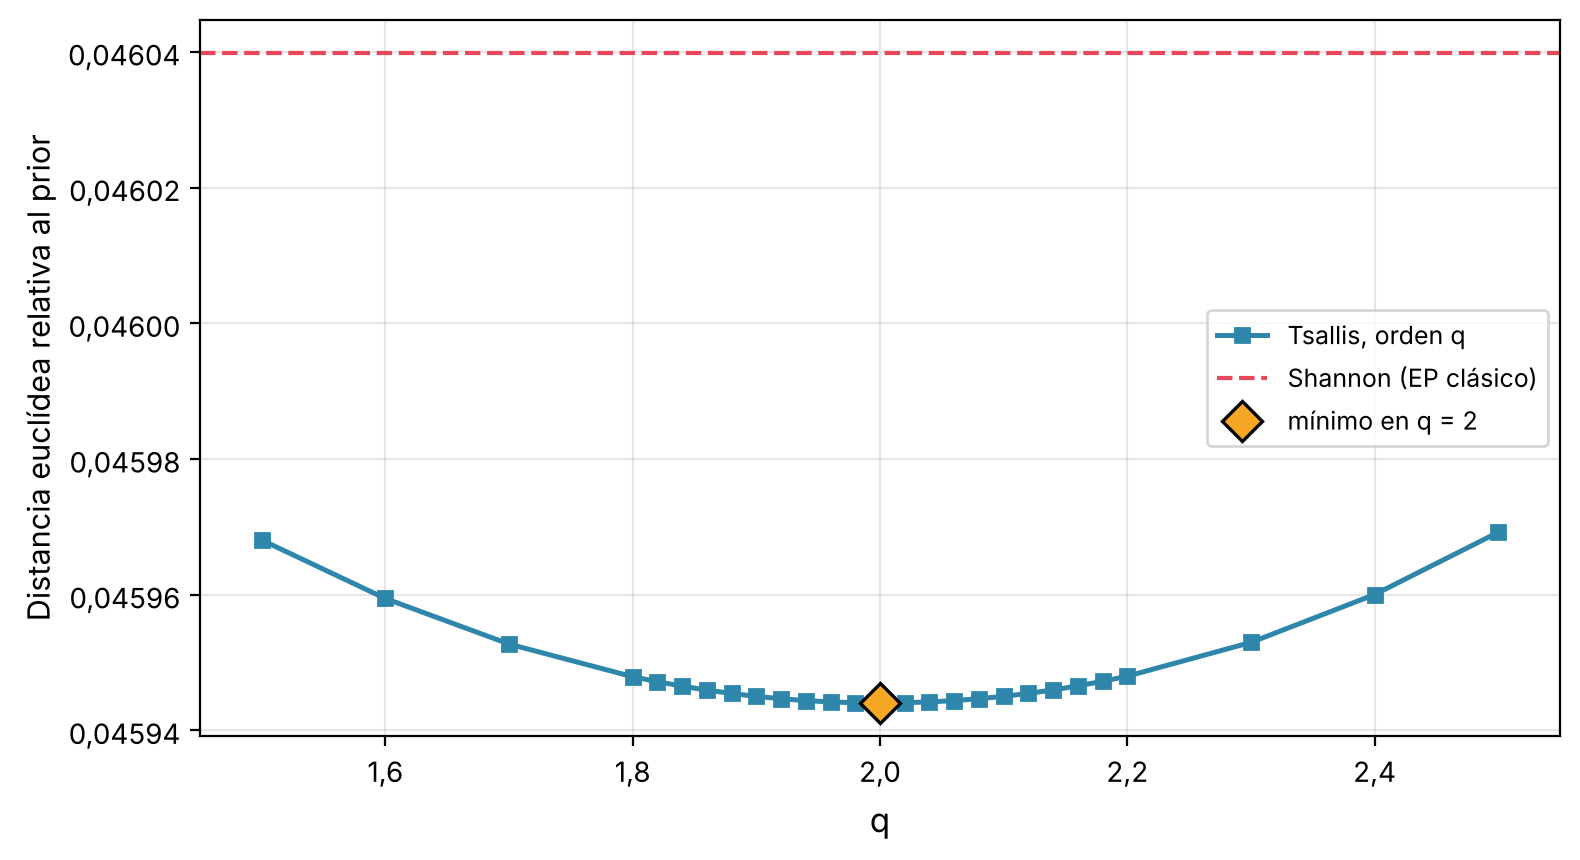
\includegraphics[width=.7\textwidth]{figs/optimal_q_zoom_es.png}
\caption{Distancia eucl\'idea relativa entre el posterior y el prior,
$\norm{\pt_{q,c} - \p}_2/\norm{\p}_2$, como funci\'on del orden $q$ (base de
\citealp{Meucci2008}, $10^5$ escenarios, un view de desigualdad,
$c=0{,}5$). La l\'inea de trazos es el EP cl\'asico. El m\'inimo en $q=2$ se
sigue de la Proposici\'on~\ref{prop:hill}.}
\label{fig:qsweep}
\end{figure}

\begin{table}[t]
\centering
\small
\caption{Distancia eucl\'idea relativa entre posterior y prior:
implementaciones en Python y en GNU Octave (base de \citealp{Meucci2008},
$10^5$ escenarios, un view de desigualdad, $c=0{,}5$). Los valores de
Octave son los registrados en el repositorio.}
\label{tab:octave}
\begin{tabular}{lcccccc}
\toprule
 & Shannon & $q=1{,}5$ & $q=1{,}9$ & $q=2{,}0$ & $q=2{,}1$ & $q=2{,}5$ \\
\midrule
Octave & 0{,}046042 & 0{,}045968 & 0{,}045945 & 0{,}045944 & 0{,}045945 & 0{,}045969 \\
Python & 0{,}046040 & 0{,}045968 & 0{,}045945 & 0{,}045944 & 0{,}045945 & 0{,}045969 \\
\bottomrule
\end{tabular}

\end{table}

\subsection{Un experimento de stress}\label{sec:separation}

Fuera de los casos de las Proposiciones~\ref{prop:local}
y~\ref{prop:jeffrey}, el de inter\'es pr\'actico es el de un view que pide un
cambio grande en alg\'un momento de la distribuci\'on.
Esta secci\'on mide ese caso sobre el panel de acciones de la
Secci\'on~\ref{sec:empirical}: $J = \nJ$ escenarios diarios para $N = \nN$
acciones, prior uniforme y confianza plena. Un solo view de desigualdad
exige que el retorno esperado de un papel (CEPU) supere su media muestral
en $k$ errores est\'andar,
$\E[X_i] \ge \hat\mu_i + k\,\hat\sigma_i/\sqrt{J}$, para $k$ entre 0 y 50.
Un error est\'andar es de \nSEday\% por d\'ia, unos \nSEann{} puntos porcentuales
por a\~no, de modo que la grilla va mucho m\'as all\'a de cualquier view que un
PM sostendr\'ia sobre un retorno esperado: $k=5$ suma \nExFive{} puntos
porcentuales por a\~no a la media hist\'orica y $k=50$ suma \nExFifty. Views de
ese tama\~no aparecen en las pruebas de stress, donde la pregunta es c\'omo
quedan los escenarios si el mercado pasa a un r\'egimen extremo, y el
experimento debe leerse en esa clave.

Para cada $k$ se calculan los posteriores de Shannon y de $q=2$ y las
carteras de
media-varianza correspondientes (sin ventas en corto, tope de 30\%,
aversi\'on al riesgo $2{,}5$). La Tabla~\ref{tab:stress} y la
Figura~\ref{fig:stress} informan los n\'umeros efectivos de escenarios de
\'ordenes 2 y 1 como fracciones de $J$, la cantidad de escenarios con
probabilidad cero bajo $q=2$, el valor en riesgo condicional (CVaR) al 5\%
del papel estresado bajo cada posterior y la distancia $\ell_1$ entre las
dos carteras.

\begin{table}[t]
\centering
\footnotesize
\caption{Experimento de stress: un view de desigualdad sobre el retorno
esperado de un papel, $k$ errores est\'andar por encima de su media muestral
($J = \nJ$, prior uniforme, confianza plena). $\Delta\mu$ es el exceso
correspondiente sobre la media hist\'orica, en puntos porcentuales por a\~no.
$N_2/J$ y $N_1/J$ son los n\'umeros efectivos de escenarios de \'ordenes 2
(Kish) y 1 (entrop\'ia) como fracciones de $J$. EP es el posterior cl\'asico (Shannon). \emph{Ceros} es la cantidad
de escenarios con probabilidad cero bajo $q=2$. CVaR es el valor en riesgo
condicional al 5\% del papel, es decir, su retorno medio en el peor 5\% de
la masa de probabilidad, en porcentaje por d\'ia ($\nCVaRprior$ bajo el
prior). $\norm{\Delta w}_1$ es la distancia $\ell_1$ entre las carteras de
media-varianza de los dos posteriores. \'Ultima fila: ranking de las \nN{}
acciones en el orden inverso al de sus medias muestrales.}
\label{tab:stress}
\begin{tabular}{rrccccrccc}
\toprule
 & & \multicolumn{2}{c}{$N_2/J$} & \multicolumn{2}{c}{$N_1/J$} & & \multicolumn{2}{c}{CVaR} & \\
\cmidrule(lr){3-4}\cmidrule(lr){5-6}\cmidrule(lr){8-9}
$k$ & $\Delta\mu$ & EP & $q=2$ & EP & $q=2$ & Ceros & EP & $q=2$ & $\norm{\Delta w}_1$ \\
\midrule
0 & 0 & 1{,}000 & 1{,}000 & 1{,}000 & 1{,}000 & 0 & $-7{,}91$ & $-7{,}91$ & 0{,}00 \\
1 & 22 & 0{,}999 & 0{,}999 & 1{,}000 & 1{,}000 & 0 & $-7{,}66$ & $-7{,}64$ & 0{,}02 \\
2 & 44 & 0{,}998 & 0{,}998 & 0{,}999 & 0{,}999 & 0 & $-7{,}44$ & $-7{,}37$ & 0{,}08 \\
5 & 110 & 0{,}987 & 0{,}987 & 0{,}993 & 0{,}993 & 1 & $-6{,}90$ & $-6{,}67$ & 0{,}08 \\
10 & 220 & 0{,}944 & 0{,}948 & 0{,}974 & 0{,}972 & 2 & $-6{,}25$ & $-5{,}66$ & 0{,}07 \\
20 & 439 & 0{,}755 & 0{,}815 & 0{,}903 & 0{,}884 & 39 & $-5{,}38$ & $-3{,}86$ & 0{,}29 \\
35 & 769 & 0{,}328 & 0{,}568 & 0{,}753 & 0{,}670 & 296 & $-4{,}59$ & $-1{,}71$ & 0{,}69 \\
50 & 1098 & 0{,}116 & 0{,}361 & 0{,}595 & 0{,}449 & 734 & $-4{,}11$ & $0{,}05$ & 1{,}18 \\
\midrule
ranking & -- & 0{,}998 & 0{,}998 & 0{,}999 & 0{,}999 & 0 & -- & -- & 0{,}00 \\
\bottomrule
\end{tabular}

\end{table}

\begin{figure}[t]
\centering
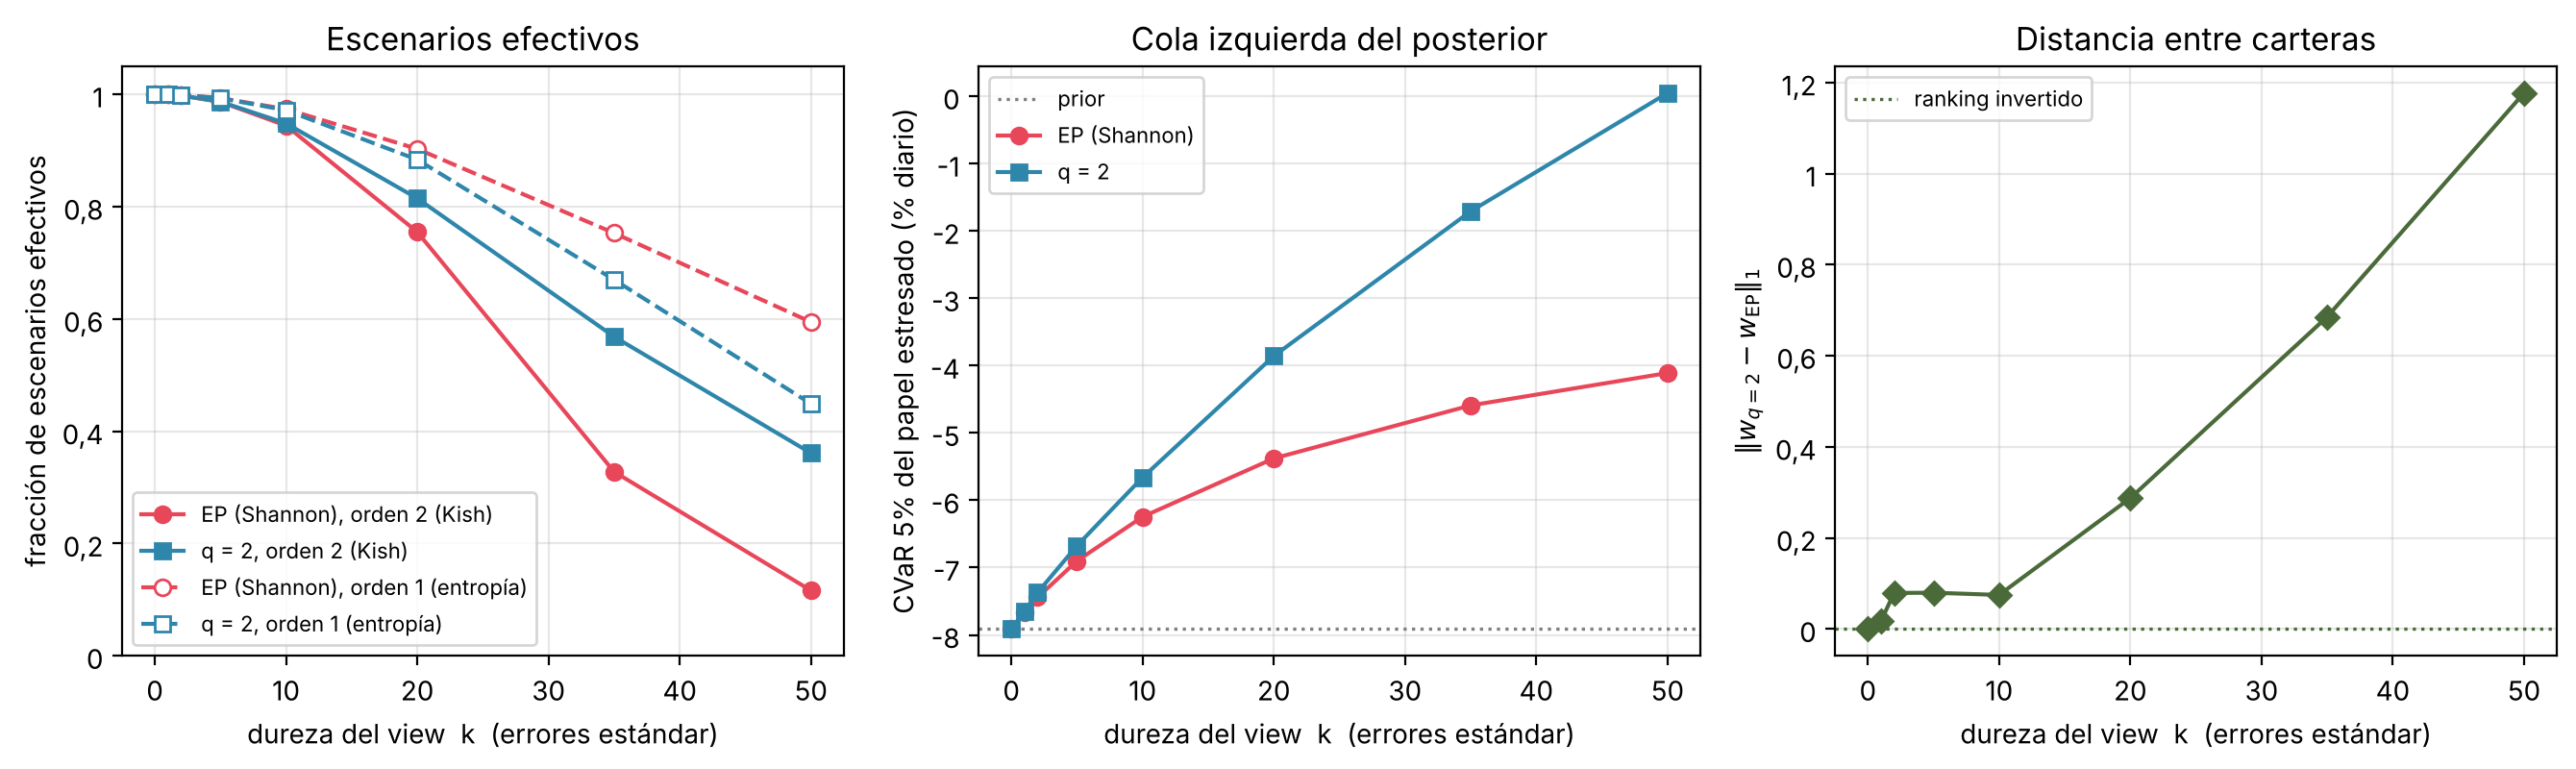
\includegraphics[width=\textwidth]{figs/qep_vs_ep_stress_es.png}
\caption{Experimento de stress de la Tabla~\ref{tab:stress}. Izquierda:
n\'umeros efectivos de escenarios de \'ordenes 2 y 1, como fracciones de $J$.
Centro: CVaR al 5\% del papel estresado bajo cada posterior. Derecha:
distancia $\ell_1$ entre las carteras de media-varianza; la l\'inea de
puntos es el ranking invertido.}
\label{fig:stress}
\end{figure}

Hasta $k=5$ los dos posteriores son iguales a los
fines pr\'acticos, como predice la Proposici\'on~\ref{prop:local}; la
diferencia entre ellos crece con $k^2$ para $k$ chico. Las carteras
difieren algo antes ($\norm{\Delta w}_1 = \nDwFive$ en $k=5$) porque el paso
de media-varianza amplifica diferencias peque\~nas en los retornos
esperados. Desde $k=5$ el papel estresado est\'a en el tope de 30\% en las
dos carteras, y la distancia entre ellas refleja c\'omo se asigna el resto.

Para $k$ m\'as grande los posteriores se separan, y cada uno es mejor seg\'un
su propia medida, como afirma la Proposici\'on~\ref{prop:hill}. En $k=20$ el
n\'umero efectivo de Kish es \nKishTTwenty{} de $J$ para $q=2$ y
\nKishSTwenty{} para Shannon; en $k=50$ es \nKishTFifty{} contra
\nKishSFifty. El n\'umero basado en la entrop\'ia va en sentido contrario:
\nEnsSFifty{} para Shannon y \nEnsTFifty{} para $q=2$ en $k=50$. La raz\'on
est\'a en la forma de la inclinaci\'on. La inclinaci\'on exponencial de Shannon
da pesos muy grandes a los pocos d\'ias con los retornos m\'as altos del papel:
el escenario de mayor peso tiene \nMaxSTwenty{} veces el peso uniforme en
$k=20$ y \nMaxSFifty{} veces en $k=50$. La inclinaci\'on lineal truncada de
$q=2$ limita esos pesos a \nMaxTTwenty{} y \nMaxTFifty{} veces el peso
uniforme y obtiene el resto de la media exigida eliminando escenarios.

Esa eliminaci\'on es el costo de $q=2$. En $k=20$ les asigna probabilidad cero a
\nZerosTwenty{} escenarios y en $k=50$ a \nZerosFifty{} de los
\nJ; son los d\'ias con los retornos m\'as bajos del papel estresado. La
cola izquierda del posterior se achica en consecuencia: el CVaR al 5\% del
papel, que es $\nCVaRprior$\% por d\'ia bajo el prior, pasa a
$\nCVaRSTwenty$\% bajo Shannon y a $\nCVaRTTwenty$\% bajo $q=2$ en $k=20$, y
a $\nCVaRSFifty$\% contra $\nCVaRTFifty$\% en $k=50$. Una medida de riesgo
calculada sobre el posterior de $q=2$ de un view fuertemente alcista
subestima entonces la p\'erdida posible respecto del EP cl\'asico, que nunca
excluye un escenario. Para un view fuertemente bajista el truncamiento
elimina, en cambio, los mejores d\'ias.

El argumento a favor del orden 2 despu\'es de la
Proposici\'on~\ref{prop:hill} era que los momentos posteriores se estiman
con menos varianza muestral. La Tabla~\ref{tab:boot} lo comprueba con un
bootstrap. Los escenarios se remuestrean con reposici\'on \nBootReps{}
veces; en cada remuestra se calculan
los dos posteriores para el mismo view, y se registran la media y la
volatilidad posteriores de la cartera equiponderada de las \nN{} acciones.
Para views suaves la dispersi\'on de esos momentos entre remuestras es casi
la misma con los dos posteriores. Para views exigentes es mucho menor con
$q=2$: en $k=20$ el desv\'io est\'andar de la media posterior es de
\nBootSdTTwenty{} puntos b\'asicos por d\'ia contra \nBootSdSTwenty{} con
Shannon, y en $k=50$ es \nBootSdTFifty{} contra \nBootSdSFifty. La
concentraci\'on del posterior de Shannon en las observaciones m\'as grandes
est\'a relacionada con el resultado de \citet{DeyJuneja2012} seg\'un el cual la
soluci\'on de Kullback--Leibler puede no existir cuando el prior tiene colas
pesadas, y el menor error muestral del miembro $\chi^2$ coincide con lo que
\citet{MakamMillossovichTsanakas2021} informan para modelos de simulaci\'on
estresados.

\begin{table}[t]
\centering
\small
\caption{Variabilidad muestral de los momentos posteriores en el
experimento de stress. Desv\'io est\'andar, entre \nBootReps{} remuestras
bootstrap de los escenarios, de la media posterior de la cartera
equiponderada (puntos b\'asicos por d\'ia), y coeficiente de variaci\'on de su
volatilidad posterior, para el view de la Tabla~\ref{tab:stress} en cada
$k$.}
\label{tab:boot}
\begin{tabular}{rcccc}
\toprule
 & \multicolumn{2}{c}{Desv\'io de la media posterior (pb)} & \multicolumn{2}{c}{CV de la volatilidad posterior} \\
\cmidrule(lr){2-3}\cmidrule(lr){4-5}
$k$ & EP & $q=2$ & EP & $q=2$ \\
\midrule
0 & 4{,}9 & 4{,}9 & 0{,}050 & 0{,}050 \\
5 & 3{,}8 & 3{,}7 & 0{,}050 & 0{,}045 \\
10 & 4{,}4 & 4{,}0 & 0{,}079 & 0{,}061 \\
20 & 8{,}3 & 4{,}8 & 0{,}163 & 0{,}093 \\
35 & 21{,}7 & 6{,}9 & 0{,}273 & 0{,}142 \\
50 & 42{,}5 & 10{,}2 & 0{,}346 & 0{,}194 \\
\bottomrule
\end{tabular}

\end{table}

Se probaron otros dos dise\~nos. Un ranking de las \nN{} acciones en
el orden inverso al de sus medias muestrales, que impone 19 desigualdades a
la vez, mueve muy poco el posterior (n\'umero efectivo de Kish \nRankEss{} de $J$
bajo los dos posteriores, $\norm{\Delta w}_1 = \nRankDw$), porque las diferencias
entre las medias diarias son chicas respecto de su error muestral: no es
la cantidad de views lo que vuelve exigente a un conjunto de views. Y un
view que multiplica por dos o por tres la volatilidad del papel, dejando
su media sin cambios, separa a la familia mucho menos que un view sobre la
media con una p\'erdida similar de muestra efectiva (n\'umero efectivo de Kish
\nVolKishTTwo{} para $q=2$ contra \nVolKishSTwo{} para Shannon con un factor
de dos,
\nVolKishTThree{} contra \nVolKishSThree{} para un factor de tres), sin
ning\'un escenario en cero. Los views sobre la probabilidad de una cola dan
posteriores id\'enticos para los dos miembros, como implica la
Proposici\'on~\ref{prop:jeffrey} para un view sobre un solo evento. El patr\'on de los n\'umeros efectivos, los ceros y el CVaR de la
Tabla~\ref{tab:stress} es el mismo cuando se estresa otro papel y para
$q = 1{,}5$ y $q = 3$; la distancia entre las carteras cambia con el papel,
porque depende tambi\'en de d\'onde queda activo el tope. Esos resultados
est\'an en el repositorio.

% ---------------------------------------------------------------------
\section{Especificaci\'on de views}\label{sec:views}
% ---------------------------------------------------------------------

La implementaci\'on tiene un solo lenguaje para los views, que se traduce a
los insumos de cada modelo: la terna $(P, Q, \Omega)$ de Black--Litterman
(BL) y las restricciones~\eqref{eq:constraints} de EP. La
Tabla~\ref{tab:views} lista los tipos.

\begin{table}[t]
\centering
\small
\caption{Tipos de views y su forma en cada modelo.}
\label{tab:views}
\begin{tabular}{lll}
\toprule
View & Restricci\'on sobre el posterior (EP) & Black--Litterman \\
\midrule
absoluto & $\E[X_i] = \mu^\ast$ & s\'i \\
relativo & $\E[X_i - X_k] = s^\ast$ & s\'i \\
ranking & $\E[X_{i_1}] \ge \E[X_{i_2}] \ge \dots$ & relativos con $s^\ast \approx 0$ \\
desigualdad (absoluta o relativa) & $\E[\cdot] \ge$ o $\le$ una cota & no \\
volatilidad & $\E[X_i^2] = \sigma^{\ast 2} + \mu_{prior}^2$, o una cota & no \\
cola & $\Pr(X_i < t) \le \pi$ o $\Pr(X_i > t) \le \pi$ & no \\
\bottomrule
\end{tabular}
\end{table}

Dos diferencias importan al comparar los modelos. BL no tiene
desigualdades: un ranking entra como una cadena de views relativos con un
spread cercano a cero, lo que dice que los retornos esperados son casi
iguales, con una incertidumbre $\Omega$; EP impone la restricci\'on de un
solo lado. Y los views sobre volatilidades o colas no tienen contraparte
en BL. La incertidumbre de los views de BL se fija a partir de la confianza
declarada $c_k$ en el view $k$ como
$\Omega_k = \frac{1-c_k}{c_k}\,\tau\, P_k \Sigma P_k^\top$, una versi\'on en
forma cerrada de la calibraci\'on por niveles de confianza de
\citet{Idzorek2007}.

% ---------------------------------------------------------------------
\section{Aplicaci\'on: acciones argentinas}\label{sec:empirical}
% ---------------------------------------------------------------------

\subsection{Datos y priors}

El universo son las 20 acciones del panel l\'ider de la bolsa de Buenos
Aires. La muestra de estimaci\'on son los retornos simples diarios en pesos
del 24 de noviembre de 2017 al 22 de septiembre de 2025, lo que da
$J = \nJ$ escenarios; el prior es uniforme. El benchmark es una cartera de
esas 20 acciones con las ponderaciones del \'indice Merval en su rebalanceo
de septiembre de 2025, que se mantiene sin rebalanceos posteriores; no es
el \'indice.
Las carteras se forman al cierre del 22 de septiembre de 2025. Tres
precios faltantes de un papel (VALO) se completan por interpolaci\'on
lineal; con ellos el panel queda completo, y la matriz de covarianzas es
la covarianza muestral.

Se usan dos priors, con los mismos escenarios y distintos retornos
esperados. El prior \emph{hist\'orico} es el conjunto de escenarios tal como
se observ\'o, de modo que los retornos esperados a priori son las medias
muestrales. El prior de \emph{equilibrio} desplaza los escenarios para que
sus medias sean los retornos impl\'icitos en el benchmark,
$\Pi = \delta\,\Sigma\, w_{bench}$, con $\delta = 2{,}5$: cada escenario se
reemplaza por $X_j - \hat\mu + \Pi$, lo que conserva las covarianzas y los
momentos superiores. BL usa el prior de equilibrio por construcci\'on, con
$\tau = 0{,}05$; con la calibraci\'on de $\Omega$ que se usa aqu\'i, que es
proporcional a $\tau$, los retornos esperados de BL no dependen de ese
valor.

Los dos priors discrepan sobre los retornos esperados. Las medias
hist\'oricas son parecidas entre papeles (entre \nMuHistMin\% y
\nMuHistMax\% por a\~no en pesos nominales), mientras que los retornos de
equilibrio son proporcionales a la covarianza con el benchmark: est\'an
entre \nPiLowMin\% y \nPiLowMax\% para ALUA, VALO y BYMA y entre
\nPiBankMin\% y \nPiBankMax\% para los cuatro bancos. Con el prior
hist\'orico un inversor de media-varianza prefiere entonces los papeles con
baja covarianza con el benchmark, y con el prior de equilibrio mantiene el
benchmark.

\subsection{Views}

Los views se basan en las opiniones que un portfolio manager de acciones
argentinas ten\'ia en septiembre de 2025 y comparti\'o con el autor: (i)
dentro del sector energ\'etico, el ranking YPFD $\succ$ PAMP $\succ$ TGSU2
$\succ$ CEPU, con confianza $0{,}70$; y (ii) cada una de las dos
energ\'eticas preferidas (YPFD y PAMP) rinde m\'as que cada uno de cuatro
bancos (GGAL, BBAR, BMA y SUPV), con confianza $0{,}50$. Las dos
afirmaciones son ordinales. En EP entran como $3 + 8 = \nIneq$
desigualdades entre retornos esperados, impuestas tal como est\'an
enunciadas. La confianza asignada a cada afirmaci\'on no se usa en EP; la
confianza parcial entra una sola vez, a trav\'es de la
mezcla con el prior con $c=0{,}5$. En BL el ranking entra como tres views
relativos con un spread cercano a cero y las ocho afirmaciones sobre bancos
como views relativos con spread cero, con las confianzas declaradas en
$\Omega$. Esa codificaci\'on no le da a BL informaci\'on sobre la direcci\'on
de los views: un view relativo con spread cero dice que dos retornos
esperados son iguales. BL podr\'ia llevar la direcci\'on con un spread
positivo, pero eso requiere un n\'umero que el PM no dio. La comparaci\'on
entre BL y EP que sigue es, entonces, una comparaci\'on entre dos
codificaciones de afirmaciones ordinales y no dice nada sobre BL con views
cuantificados. Los views se escribieron en el c\'odigo despu\'es del final del
per\'iodo de evaluaci\'on, de modo que el ejercicio ilustra el m\'etodo y no es
una prueba de los pron\'osticos del PM.

Con el prior hist\'orico solo una de las \nIneq{} desigualdades queda activa
(PAMP sobre TGSU2), y con el prior de equilibrio quedan activas
\nActiveEq, porque los retornos de equilibrio ordenan a los bancos por
encima de las energ\'eticas. En los dos casos los views son suaves en el
sentido de la Secci\'on~\ref{sec:optimalq}: antes de mezclar con el prior,
el tama\~no muestral efectivo de Kish del posterior de EP es el
\nEssHist\% de $J$ con el prior hist\'orico y el \nEssEq\% con el prior de
equilibrio, y ning\'un retorno esperado
se mueve m\'as de \nShiftEq{} puntos porcentuales por a\~no.

\subsection{Carteras}

Para cada prior se calculan cuatro carteras con el mismo paso de
media-varianza (sin ventas en corto, aversi\'on al riesgo $\delta = 2{,}5$,
tope de 30\% por papel): una sin views y una para cada regla de
actualizaci\'on, BL, EP y EP con $q = 2$. Para el prior hist\'orico la f\'ormula
de BL se aplica con las medias muestrales en lugar de $\Pi$. Las carteras de BL
usan los retornos esperados de BL con la matriz de covarianzas del prior, y
las de EP usan las medias y covarianzas de los escenarios bajo el
posterior. Sin views el
prior de equilibrio reproduce el benchmark, as\'i que el benchmark es la
cartera sin views de ese prior. La Tabla~\ref{tab:weights} informa las
ponderaciones. El tope no queda activo en ninguna de ellas.

\begin{table}[t]
\centering
\footnotesize
\caption{Ponderaciones de las carteras (\%) al 22 de septiembre de 2025,
por prior y regla de actualizaci\'on. Retornos simples, sin ventas en corto,
tope de 30\%, $\delta = 2{,}5$, $\tau = 0{,}05$, confianza global $0{,}5$
para EP. \emph{Sin views} es la cartera de media-varianza de cada prior;
para el prior de equilibrio es el benchmark. La \'ultima fila es la distancia
$\ell_1$ a la cartera sin views del mismo prior.}
\label{tab:weights}
\begin{tabular}{lrrrrrrrr}
\toprule
 & \multicolumn{4}{c}{Prior de equilibrio} & \multicolumn{4}{c}{Prior hist\'orico} \\
\cmidrule(lr){2-5}\cmidrule(lr){6-9}
 & Sin views & BL & EP & $q=2$ & Sin views & BL & EP & $q=2$ \\
\midrule
ALUA & 2{,}68 & 2{,}95 & 3{,}04 & 3{,}03 & 16{,}39 & 15{,}32 & 16{,}28 & 16{,}29 \\
BBAR & 5{,}20 & 0{,}00 & 2{,}65 & 2{,}64 & 0{,}00 & 0{,}00 & 0{,}00 & 0{,}00 \\
BMA & 8{,}01 & 0{,}00 & 1{,}01 & 1{,}01 & 0{,}00 & 0{,}00 & 0{,}00 & 0{,}00 \\
BYMA & 4{,}72 & 4{,}45 & 4{,}40 & 4{,}41 & 21{,}50 & 24{,}28 & 21{,}63 & 21{,}63 \\
CEPU & 6{,}23 & 3{,}46 & 3{,}53 & 3{,}55 & 0{,}00 & 0{,}00 & 0{,}00 & 0{,}00 \\
COME & 1{,}36 & 1{,}22 & 1{,}34 & 1{,}34 & 0{,}00 & 0{,}00 & 0{,}00 & 0{,}00 \\
CRES & 2{,}68 & 2{,}72 & 2{,}87 & 2{,}86 & 2{,}15 & 3{,}11 & 2{,}21 & 2{,}22 \\
EDN & 1{,}23 & 1{,}05 & 1{,}07 & 1{,}09 & 0{,}00 & 0{,}00 & 0{,}00 & 0{,}00 \\
GGAL & 15{,}04 & 7{,}85 & 13{,}45 & 13{,}46 & 0{,}00 & 0{,}00 & 0{,}00 & 0{,}00 \\
LOMA & 3{,}47 & 3{,}39 & 3{,}30 & 3{,}35 & 0{,}00 & 0{,}00 & 0{,}00 & 0{,}00 \\
METR & 0{,}87 & 0{,}28 & 0{,}61 & 0{,}60 & 0{,}00 & 0{,}00 & 0{,}00 & 0{,}00 \\
PAMP & 14{,}68 & 27{,}05 & 23{,}26 & 23{,}24 & 0{,}00 & 11{,}09 & 7{,}23 & 7{,}23 \\
SUPV & 2{,}74 & 0{,}00 & 0{,}00 & 0{,}00 & 0{,}00 & 0{,}00 & 0{,}00 & 0{,}00 \\
TECO2 & 2{,}19 & 2{,}20 & 2{,}35 & 2{,}31 & 0{,}00 & 0{,}00 & 0{,}00 & 0{,}00 \\
TGNO4 & 1{,}17 & 1{,}14 & 1{,}11 & 1{,}10 & 0{,}00 & 0{,}00 & 0{,}00 & 0{,}00 \\
TGSU2 & 5{,}64 & 10{,}69 & 8{,}00 & 8{,}02 & 18{,}45 & 4{,}69 & 11{,}00 & 11{,}00 \\
TRAN & 1{,}23 & 1{,}28 & 0{,}93 & 0{,}95 & 0{,}00 & 0{,}71 & 0{,}00 & 0{,}00 \\
TXAR & 5{,}02 & 4{,}98 & 5{,}05 & 5{,}05 & 3{,}76 & 5{,}42 & 3{,}81 & 3{,}81 \\
VALO & 1{,}28 & 1{,}37 & 1{,}53 & 1{,}51 & 21{,}11 & 22{,}72 & 21{,}15 & 21{,}15 \\
YPFD & 14{,}55 & 23{,}91 & 20{,}49 & 20{,}47 & 16{,}63 & 12{,}65 & 16{,}68 & 16{,}68 \\
\midrule
$\norm{w - w_{\text{sin views}}}_1$ & -- & 0{,}54 & 0{,}36 & 0{,}36 & -- & 0{,}38 & 0{,}15 & 0{,}15 \\
\bottomrule
\end{tabular}

\end{table}

La elecci\'on de $q$ no importa: las
carteras de EP y de $q=2$ difieren en $\norm{\Delta w}_1 = \nLoneQhist$ con
el prior hist\'orico y en \nLoneQeq{} con el prior de equilibrio, como cabe
esperar con views suaves. El prior es lo que m\'as importa. Las dos carteras
sin views est\'an a una distancia de \nLonePrior{} entre s\'i, sobre un m\'aximo
de 2, porque la cartera del prior hist\'orico se concentra en papeles que
pesan poco en el benchmark. Los views mueven la cartera menos: \nLoneEPhist{} para EP y
\nLoneBLhist{} para BL con el prior hist\'orico, \nLoneEPeq{} y \nLoneBLeq{}
con el prior de equilibrio. Con los dos priors BL mueve la cartera m\'as que EP, y con
el prior de equilibrio saca de la cartera a tres de los cuatro bancos. La
diferencia viene de c\'omo entra la confianza. BL trata las once
afirmaciones como evidencias separadas, cada una con su confianza, y cada
una lleva un spread hacia cero; EP impone las desigualdades y despu\'es se
mezcla una sola vez con el prior, lo que deja los retornos esperados m\'as o
menos a mitad de camino. Con $c=1$ en EP el orden se invierte con el prior
de equilibrio: EP mueve la cartera en \nLoneEPeqFull{} y BL en \nLoneBLeq{}
(Ap\'endice~\ref{app:robust}).

\subsection{Evaluaci\'on fuera de muestra}

Las carteras se mantienen desde el cierre del 22 de septiembre de 2025
hasta el 20 de marzo de 2026, \nDays{} ruedas posteriores al final de la
muestra de estimaci\'on, sin rebalanceo. La Tabla~\ref{tab:oos} informa los
resultados y la Figura~\ref{fig:oos} las trayectorias. Los retornos son
nominales, en pesos, y el ratio de Sharpe se calcula con tasa libre de
riesgo cero; con las tasas de inter\'es en pesos del per\'iodo su nivel est\'a
sobrestimado para todas las carteras, y solo tienen sentido las
comparaciones entre ellas.

\begin{table}[t]
\centering
\footnotesize
\caption{Resultados fuera de muestra, 22 de septiembre de 2025 a 20 de
marzo de 2026 (\nDays{} ruedas), \emph{buy and hold}. El retorno es el acumulado en la
ventana, en pesos; volatilidad anualizada con 252 d\'ias; ratio de Sharpe con tasa libre de
riesgo cero; \emph{tracking error} (TE) y beta respecto del benchmark. La
\'ultima columna es la diferencia de ratio de Sharpe con la cartera sin views
del mismo prior y su intervalo de confianza de 95\% por bootstrap circular
en bloques (bloques de 5 d\'ias, 10.000 r\'eplicas). La cartera de m\'inima
varianza se calcula con las mismas restricciones y est\'a en el tope de 30\%
en un papel.}
\label{tab:oos}
\begin{tabular}{lrrrrrrl}
\toprule
 & Retorno & Vol. & Sharpe & Ca\'ida m\'ax. & TE & Beta & $\Delta$ Sharpe \\
 & (\%) & (\%) & & (\%) & (\%) & & [intervalo de 95\%] \\
\midrule
\multicolumn{8}{l}{\emph{Prior de equilibrio}} \\
\quad Sin views (benchmark) & 49{,}0 & 47{,}6 & 1{,}97 & $-21{,}1$ & -- & -- & -- \\
\quad BL & 48{,}1 & 40{,}8 & 2{,}20 & $-16{,}7$ & 10{,}4 & 0{,}84 & $+0{,}23$ $[-0{,}38;\, +0{,}99]$ \\
\quad EP & 47{,}6 & 42{,}8 & 2{,}10 & $-18{,}3$ & 6{,}9 & 0{,}89 & $+0{,}13$ $[-0{,}26;\, +0{,}59]$ \\
\quad EP, $q=2$ & 47{,}6 & 42{,}8 & 2{,}10 & $-18{,}3$ & 6{,}9 & 0{,}89 & $+0{,}13$ $[-0{,}26;\, +0{,}59]$ \\
\addlinespace
\multicolumn{8}{l}{\emph{Prior hist\'orico}} \\
\quad Sin views & 67{,}9 & 36{,}0 & 3{,}18 & $-17{,}4$ & 20{,}9 & 0{,}69 & -- \\
\quad BL & 68{,}7 & 35{,}5 & 3{,}24 & $-17{,}2$ & 22{,}8 & 0{,}66 & $+0{,}06$ $[-0{,}26;\, +0{,}35]$ \\
\quad EP & 67{,}2 & 35{,}5 & 3{,}19 & $-17{,}5$ & 21{,}5 & 0{,}68 & $+0{,}02$ $[-0{,}13;\, +0{,}14]$ \\
\quad EP, $q=2$ & 67{,}2 & 35{,}5 & 3{,}19 & $-17{,}5$ & 21{,}5 & 0{,}68 & $+0{,}02$ $[-0{,}13;\, +0{,}14]$ \\
\addlinespace
\multicolumn{8}{l}{\emph{Carteras de referencia}} \\
\quad Equiponderada & 53{,}8 & 49{,}7 & 2{,}04 & $-21{,}8$ & 8{,}5 & 1{,}03 & -- \\
\quad M\'inima varianza & 62{,}7 & 38{,}7 & 2{,}81 & $-21{,}3$ & 23{,}1 & 0{,}71 & -- \\
\bottomrule
\end{tabular}

\end{table}

\begin{figure}[t]
\centering
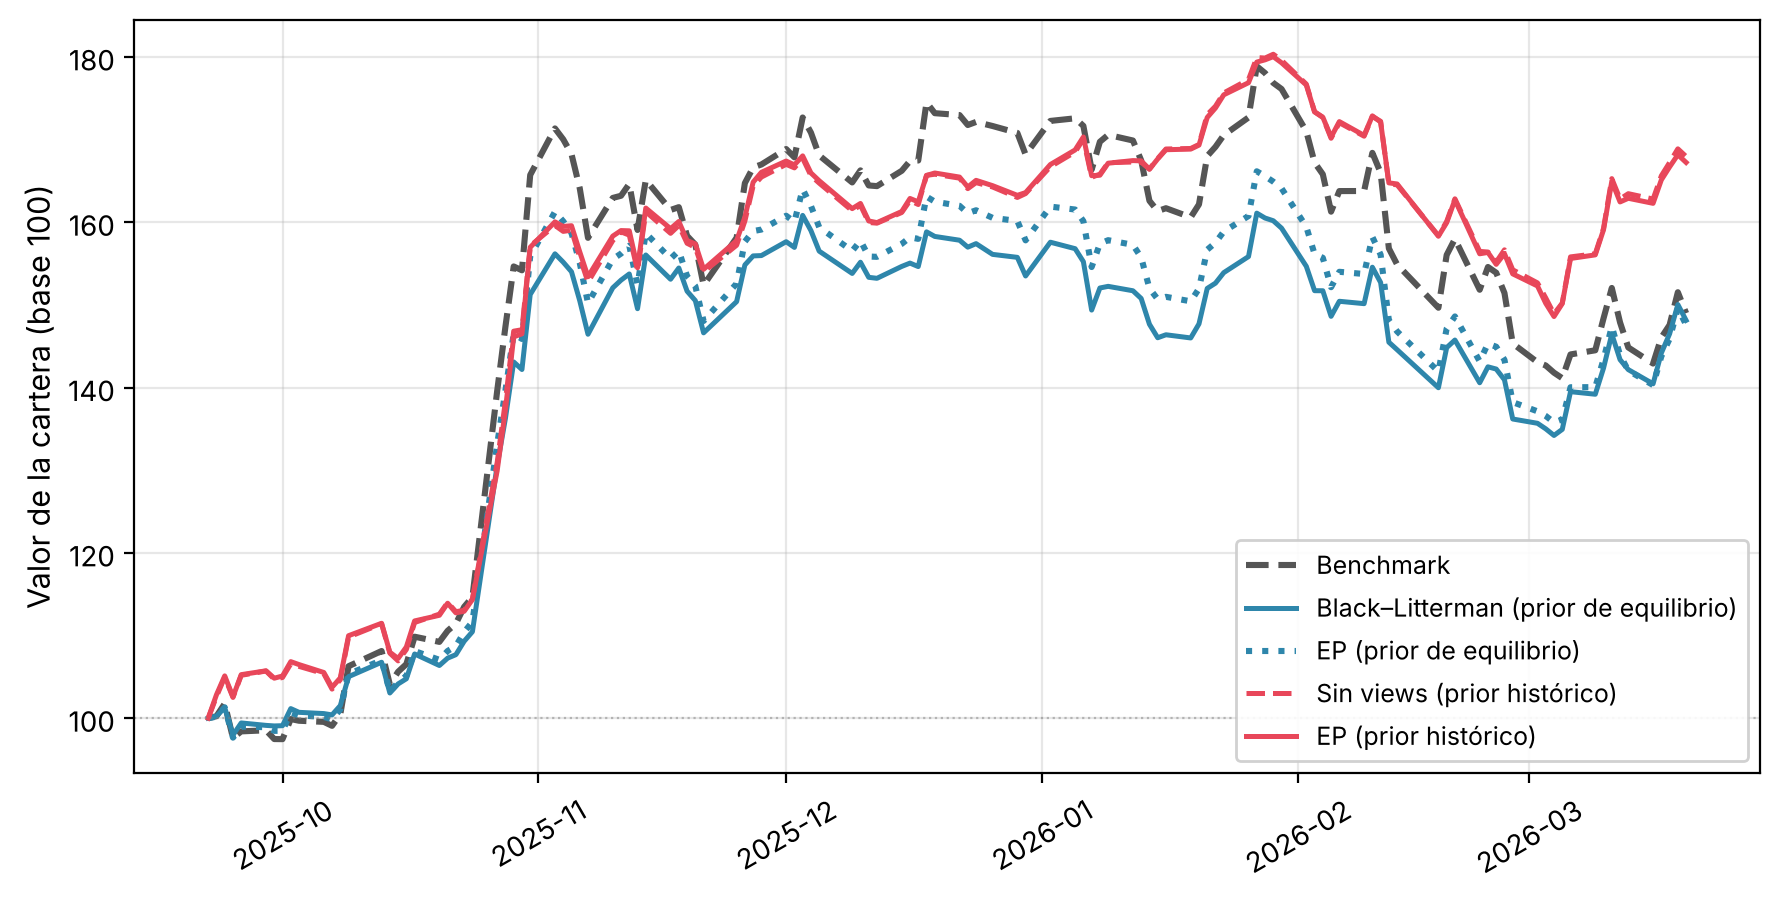
\includegraphics[width=.85\textwidth]{figs/oos_evolution_es.png}
\caption{Valor de las carteras, 22 de septiembre de 2025 a 20 de marzo de
2026 (base 100, \emph{buy and hold}). Las carteras de $q=2$ coinciden con
las de EP y se omiten, igual que BL con el prior hist\'orico y las dos
carteras de referencia; con el prior hist\'orico las carteras de EP y sin
views son casi indistinguibles.}
\label{fig:oos}
\end{figure}

Las carteras se dividen en dos grupos seg\'un el prior. Las construidas
sobre el prior de equilibrio se comportan como el benchmark: retornos
acumulados entre \nRetEPeq\% y \nRetBench\% y ratios de Sharpe entre
\nShBench{} y \nShBL. Las construidas sobre el prior hist\'orico rinden
entre \nRetEP\% y \nRetBLhist\% con unas tres cuartas partes de la
volatilidad del benchmark, y sus ratios de Sharpe est\'an entre \nShMVhist{} y
\nShBLhist. La cartera sin views ya tiene un ratio de Sharpe de
\nShMVhist. Los papeles de baja volatilidad rindieron bien en el per\'iodo:
la cartera de m\'inima varianza, que no usa retornos esperados, tiene un
ratio de Sharpe de \nShMinVar{} y la cartera equiponderada uno de \nShEW.
Dos papeles sobre los que el PM no expres\'o ning\'un view, VALO y BYMA,
suman \nContribTop{} puntos porcentuales al retorno de la cartera sin views
del prior hist\'orico respecto del benchmark, m\'as que toda la diferencia de
\nContribTotal{} puntos entre las dos.

Dentro de cada prior los views agregan poco. Con el prior hist\'orico la
cartera de EP tiene un ratio de Sharpe $\nBootEPdiff$ mayor que la cartera
sin views, con un intervalo de 95\% de $[\nBootEPlo;\, \nBootEPhi]$. Con el
prior de equilibrio BL mejora al benchmark en $\nBootBLdiff$
($[\nBootBLlo;\, \nBootBLhi]$) y EP en $\nBootEPeqdiff$
($[\nBootEPeqlo;\, \nBootEPeqhi]$), en los dos casos con menor volatilidad y
un retorno algo menor. Ninguna de estas diferencias se puede distinguir de
cero con \nDays{} observaciones. La diferencia entre las dos carteras sin
views es mayor, $\nBootPriordiff$ de ratio de Sharpe, pero est\'a en el
l\'imite de lo que la ventana permite detectar. Su intervalo es
$[\nBootPriorlo;\, \nBootPriorhi]$ con bloques de cinco d\'ias, y con
bloques de 1, 3, 5, 10 y 20 d\'ias y otras diez semillas del bootstrap para
cada largo el extremo inferior
queda entre $\nBootPriorLoMin$ y $\nBootPriorLoMax$. En total se calcularon
diez intervalos, sin ajuste por comparaciones m\'ultiples. BL y EP est\'an
m\'as cerca entre s\'i dentro de un prior que cualquiera de los dos de su
contraparte con el otro prior.

Una comparaci\'on directa de BL con el prior de equilibrio y EP sobre
escenarios hist\'oricos, que es como se suelen correr los dos m\'etodos,
mostrar\'ia a EP adelante por $\nBootUsualdiff$ de ratio de Sharpe (\nShEP{}
contra \nShBL, con un intervalo de $[\nBootUsuallo;\, \nBootUsualhi]$). El
dise\~no descompone esa brecha: $\nBootPriordiff$ es la diferencia entre las
dos carteras sin views, y los efectos de los views dentro de cada prior
($\nBootEPdiff$ para EP y $\nBootBLdiff$ para BL) explican el resto. La
f\'ormula de BL aplicada al prior hist\'orico rinde tanto como EP, y EP
aplicado al prior de equilibrio no rinde m\'as que BL. Dada la codificaci\'on
de los views, en la que BL lleva los spreads hacia cero y no tiene
direcci\'on, esto compara dos codificaciones en una ventana y no ordena las
dos reglas.

\subsection{Limitaciones y robustez}\label{sec:limitations}

La evaluaci\'on abarca una sola ventana de seis meses en un solo mercado, as\'i que
describe un episodio. La ventana no se eligi\'o de antemano, los views se
escribieron en el c\'odigo despu\'es de ella, y el per\'iodo incluye la elecci\'on
legislativa de octubre de 2025. Un solo d\'ia explica buena parte del nivel
de los ratios de Sharpe: el \nExtDay, la primera rueda despu\'es de la
elecci\'on, el benchmark subi\'o \nExtBench\% y la cartera sin views del prior
hist\'orico \nExtMVhist\%. Sin ese d\'ia sus ratios de Sharpe son
\nShBenchEx{} y \nShMVhistEx; el orden de los dos priors no depende de
\'el. El buen desempe\~no del prior hist\'orico es
el desempe\~no de unos pocos papeles con baja covarianza con el benchmark en
ese episodio y depende de la muestra de estimaci\'on: con los escenarios de
los \'ultimos cinco o tres a\~nos en lugar de toda la muestra, la cartera sin
views del prior hist\'orico tiene un ratio de Sharpe entre \nShWinNVmin{} y
\nShWinNVmax, cercano al del benchmark.

Un placebo confirma que la ventana contiene poca informaci\'on sobre los
views. Reemplazarlos por sus opuestos (el ranking inverso y los bancos por
encima de las energ\'eticas) deja los ratios de Sharpe de las carteras de BL sin cambios hasta el
segundo decimal, porque un ranking escrito como spreads cercanos a cero no tiene
direcci\'on, y da carteras de EP con ratios de Sharpe de \nShPlaceboEP{} con
el prior hist\'orico y de \nShPlaceboEPeq{} con el prior de equilibrio,
contra \nShEP{} y \nShEPeq{} con los views del PM. Con el prior de
equilibrio los views opuestos ya se cumplen bajo el prior, as\'i que esa
cartera es el benchmark.

No se consideran costos de transacci\'on. Pasar del benchmark a la cartera
de EP con el prior hist\'orico requiere operar el \nTurnEP{} del valor de la
cartera, contando compras y ventas; a 50 puntos b\'asicos por lado esto
cuesta alrededor de \nCostEP\% una sola vez, lo que es poco frente a las
diferencias de la Tabla~\ref{tab:oos}. Con una tasa libre de riesgo de
30\% anual en lugar de cero los ratios de Sharpe de todas las carteras
bajan, a \nShBenchRf{} para el benchmark y a \nShMVhistRf{} para la cartera
sin views del prior hist\'orico, y el orden de las ocho carteras del
dise\~no no cambia.

Tres rasgos de los datos matizan el desempe\~no del prior hist\'orico. El
universo es el conjunto de papeles que estaban en el \'indice en la fecha de
formaci\'on, de modo que las medias hist\'oricas son las de papeles
seleccionados al final de la muestra. Los tres papeles que suman el
\nWIlliq\% de la cartera sin views (VALO, BYMA y ALUA) tienen retorno cero
en entre el \nZeroIlliqMin\% y el \nZeroIlliqMax\% de las ruedas de la
muestra de estimaci\'on, contra entre el \nZeroLiqMin\% y el
\nZeroLiqMax\% de YPFD y los cuatro bancos. La negociaci\'on infrecuente
baja las covarianzas medidas, que es lo que el optimizador premia con ese
prior, y el costo supuesto m\'as arriba no incluye el impacto en precios de
posiciones de ese tama\~no. Y los retornos son nominales, en pesos, sobre
una muestra con inflaci\'on alta y variable; no se corri\'o ninguna variante
en d\'olares ni en t\'erminos reales.

El Ap\'endice~\ref{app:robust} detalla las variantes anteriores y otras que cambian
un supuesto por vez: la confianza, el orden $q$, el tope, la aversi\'on al
riesgo, retornos logar\'itmicos en lugar de simples, rebalanceo diario en
lugar de \emph{buy and hold} y la codificaci\'on de los views sobre bancos
como igualdades con objetivos a mitad de camino del prior, que fue la
primera versi\'on de este ejercicio. Con el prior hist\'orico, el ratio de
Sharpe de EP difiere del de su cartera sin views en un valor de entre
$\nRobMin$ y $\nRobMax$ en todas las variantes, y las carteras de EP y de
$q=2$ difieren en menos de \nRobQmax{} en distancia $\ell_1$. Con el prior
de equilibrio los rangos son m\'as amplios: EP supera al benchmark en un
valor de entre cero y $\nRobEqMax$, el m\'aximo con confianza plena, y las
dos carteras de EP difieren en menos de \nRobQmaxEq. La codificaci\'on con igualdades no tiene soluci\'on
con el prior de equilibrio, porque las igualdades de las dos energ\'eticas implican, al
restarlas, que la diferencia entre los retornos esperados de YPFD y PAMP
es la mitad de su valor a priori, lo que
contradice el ranking cuando el prior ordena primero a PAMP.

% ---------------------------------------------------------------------
\section{Extensi\'on a renta fija}\label{sec:bonds}
% ---------------------------------------------------------------------

Para bonos el invariante natural es el cambio de rendimiento, $\Delta y$,
y no el retorno de precio, cuya distribuci\'on cambia a medida que el bono se
acerca al vencimiento. El repositorio incluye una versi\'on del
procedimiento que corre EP sobre escenarios de cambios de rendimiento y
optimiza sobre los retornos de precio que implican. Esta secci\'on la
describe; en este trabajo no se informan resultados emp\'iricos para bonos.

Con duration modificada $D_t$ y convexidad $C_t$, el retorno de precio se
aproxima por
\begin{equation}\label{eq:duration}
\frac{\Delta P_t}{P_{t}} \;\approx\; -\,D_{t}\,\Delta y_t \;+\; \tfrac{1}{2}\,C_{t}\,(\Delta y_t)^2,
\end{equation}
con tres opciones: una duration constante (la de la fecha de formaci\'on),
una duration que cambia en el tiempo y esta \'ultima con el t\'ermino de
convexidad. La transformaci\'on da solo el retorno de precio; no incluye el
devengamiento. Los views se enuncian sobre $\Delta y$ con los tipos de la
Tabla~\ref{tab:views}. Un view de que el rendimiento del bono $i$ caer\'a m\'as que el del bono
$k$ es $\E[\Delta y_i] \le \E[\Delta y_k]$, de modo que un ranking de bonos
por retorno esperado tiene el orden inverso cuando se escribe en t\'erminos
de rendimientos. Con durations distintas el orden de los cambios de
rendimiento no es el de los retornos de precio, y un view sobre desempe\~no
relativo conviene escribirlo sobre los retornos de precio transformados,
que tambi\'en son funciones de los escenarios. Un view de
cola acota la probabilidad de una suba grande del rendimiento,
$\Pr(\Delta y_i > t) \le \pi$.

Los paneles de bonos soberanos emergentes suelen estar desbalanceados,
porque los bonos emitidos hace poco tienen historias cortas. Para esos
paneles el repositorio incluye un estimador de la matriz de covarianzas que
trabaja par por par sobre las fechas en que se observan las dos
series, con un m\'inimo de observaciones, y que vuelve semidefinido
positivo el resultado, cuando hace falta, con las proyecciones alternadas
de \citet{Higham2002}; los escenarios para EP son entonces las fechas en
que se observan todas las series. Ning\'un resultado de este trabajo
depende de \'el: el panel de acciones de la
Secci\'on~\ref{sec:empirical} est\'a completo.

% ---------------------------------------------------------------------
\section{Conclusi\'on}\label{sec:conclusion}
% ---------------------------------------------------------------------

Entropy Pooling se puede correr con cualquier miembro de la familia de
Tsallis al costo de resolver un problema dual con una variable por view.
Con prior uniforme cada miembro maximiza el n\'umero efectivo de escenarios
de su propio orden. El EP cl\'asico maximiza el n\'umero basado en la entrop\'ia
y conserva todos los escenarios; $q=2$ maximiza el tama\~no muestral efectivo
de Kish, que determina la varianza muestral de los momentos posteriores, y
es la proyecci\'on eucl\'idea del prior sobre el conjunto de distribuciones
que cumplen los views.

Para la mayor\'ia de los views la elecci\'on no tiene consecuencias. Los
miembros de la familia coinciden a primer orden en el tama\~no de los views
y dan posteriores id\'enticos para views sobre la probabilidad de un evento.
Difieren para views que exigen un cambio grande en alg\'un momento de la distribuci\'on, como en las
pruebas de stress, y ah\'i la elecci\'on es una disyuntiva: $q=2$ evita que el
posterior se concentre en unos pocos escenarios extremos, y lo hace
excluyendo los escenarios que contradicen el view, lo que reduce el riesgo
de cola que muestra el posterior. Cu\'al de los dos conviene depende de si
el posterior se va a usar para estimar momentos o para medir riesgo.

En la aplicaci\'on a acciones argentinas los views de un profesional del
mercado son suaves, las dos versiones de EP dan la misma cartera, y la
brecha fuera de muestra entre EP y Black--Litterman es la brecha entre sus
priors, en una ventana demasiado corta para establecer estad\'isticamente
cualquiera de las diferencias. Una comparaci\'on entre Black--Litterman y
Entropy Pooling en la que cada m\'etodo usa su prior habitual mide tambi\'en
la diferencia entre los priors, y para separarlas hace falta un dise\~no
que mantenga fijo el prior. Quedan pendientes dos
extensiones: una evaluaci\'on sobre muchas fechas de
formaci\'on con views registrados de antemano y la aplicaci\'on a renta fija.

% ---------------------------------------------------------------------
\section*{Declaraciones}
% ---------------------------------------------------------------------

\paragraph{Financiamiento.} Este trabajo no recibi\'o financiamiento
externo.

\paragraph{Conflictos de inter\'es.} El autor trabaja en la industria de
administraci\'on de activos. Las opiniones expresadas son propias y no
representan las de su empleador. Pablo J.~Escapa comparti\'o los views de
renta variable a t\'itulo personal y no particip\'o del an\'alisis.

\paragraph{Disponibilidad de datos y c\'odigo.} El c\'odigo que genera todas
las tablas y figuras est\'a disponible en
\begin{center}
\url{https://github.com/rodrigocorvalan93/non_extensive_q_entropy_pooling}
\end{center}
y el README indica qu\'e script produce cada resultado. El historial de
commits fecha en marzo de 2026 el marco, sus implementaciones en Octave y
en Python, el barrido de $q$ y la aplicaci\'on al Merval. La base de escenarios
de la Secci\'on~\ref{sec:numerics} es la que se distribuye con
\citet{Meucci2008}. Los precios diarios de las acciones y las ponderaciones
del benchmark son de Bloomberg, y su redistribuci\'on est\'a sujeta a los
t\'erminos de su licencia. El repositorio documenta el formato de los
archivos de entrada e incluye la salida de cada paso, a partir de la cual
se generan las tablas sin los datos de precios.

\paragraph{Aviso.} Este es un trabajo de investigaci\'on acad\'emica. No
constituye asesoramiento de inversi\'on ni una oferta de compra o venta de
ning\'un valor negociable. Las carteras que se informan ilustran un m\'etodo y
no son recomendaciones, y los resultados fuera de muestra abarcan una sola
ventana y no anticipan rendimientos futuros.

% ---------------------------------------------------------------------
\appendix
\section{Derivaciones del dual}\label{app:dual}
% ---------------------------------------------------------------------

\paragraph{Shannon.} El lagrangiano de~\eqref{eq:primal} con $D = D_{KL}$ es
\[
L = \sum_j x_j(\ln x_j - \ln p_j) + \boldsymbol{\lambda}^\top(A\x - \mathbf{b})
+ \boldsymbol{\nu}^\top(A_{eq}\x - \mathbf{b}_{eq}),
\qquad \boldsymbol{\lambda} \ge 0 .
\]
Su derivada respecto de $x_j$ es $\ln x_j - \ln p_j + 1 + z_j$, con
$\mathbf{z} = A^\top\boldsymbol{\lambda} + A_{eq}^\top\boldsymbol{\nu}$.
Igualarla a cero da~\eqref{eq:kkt-shannon}. La soluci\'on es positiva, as\'i
que la restricci\'on $x_j \ge 0$ nunca queda activa.

\paragraph{Tsallis, $q>1$.} Con $D = D_q$,
$\partial L/\partial x_j = \frac{q}{q-1}\,(x_j/p_j)^{q-1} + z_j$. Si
$z_j < 0$ la derivada se anula en
$(x_j/p_j)^{q-1} = -\frac{q-1}{q}\,z_j > 0$, que es la soluci\'on interior
de~\eqref{eq:kkt-tsallis}. Si $z_j \ge 0$ la derivada es positiva para todo
$x_j > 0$, as\'i que el m\'inimo de $L$ sobre $x_j \ge 0$ est\'a en $x_j = 0$.
Los dos casos juntos dan~\eqref{eq:kkt-tsallis}. Para $0<q<1$ la
derivada tiende a $-\infty$ cuando $x_j \to 0$, de modo que el m\'inimo es
interior y requiere $z_j > 0$:
$x_j = p_j\,[(1-q)\,z_j/q]^{-1/(1-q)}$, sin truncamiento.

\paragraph{Funci\'on dual.} Sea
$\x(\boldsymbol{\lambda},\boldsymbol{\nu})$ el minimizador de $L$ sobre
$\x \ge 0$. La funci\'on dual
$g(\boldsymbol{\lambda},\boldsymbol{\nu}) = L\big(\x(\boldsymbol{\lambda},\boldsymbol{\nu}),
\boldsymbol{\lambda},\boldsymbol{\nu}\big)$ es c\'oncava, por ser un m\'inimo punto a punto de
funciones afines en los multiplicadores, y su gradiente es
$\big(A\x - \mathbf{b},\; A_{eq}\x - \mathbf{b}_{eq}\big)$ evaluado en
$\x(\boldsymbol{\lambda},\boldsymbol{\nu})$. En un m\'aximo de $g$ sujeto a
$\boldsymbol{\lambda} \ge 0$ se cumplen las restricciones de igualdad, se
cumplen las de desigualdad, y $\lambda_i (A\x - \mathbf{b})_i = 0$ para cada
desigualdad, de modo que $\x(\boldsymbol{\lambda},\boldsymbol{\nu})$
satisface las condiciones de optimalidad de~\eqref{eq:primal} y es el
posterior.

% ---------------------------------------------------------------------
\section{Demostraciones y otras propiedades de la familia}\label{app:proofs}
% ---------------------------------------------------------------------

\paragraph{Demostraci\'on de la Proposici\'on~\ref{prop:local}.} Para $\x$
cercano a $\p$ las restricciones de no negatividad no est\'an activas, y las
condiciones de optimalidad son $\varphi'(x_j/p_j) + z_j = 0$ con
$\mathbf{z} = A_{eq}^\top \boldsymbol{\nu}$, junto con los views. Como
$\varphi''(1) > 0$, $\varphi'$ tiene una inversa diferenciable $\psi$ cerca
de $\varphi'(1)$, con $\psi'(\varphi'(1)) = 1/\varphi''(1)$, y
$x_j = p_j\,\psi(-z_j)$. En $\varepsilon = 0$ la soluci\'on es $\x = \p$,
con $z_j = -\varphi'(1)$ para todo $j$; esto es
$\mathbf{z} = A_{eq}^\top \boldsymbol{\nu}^0$ para el vector
$\boldsymbol{\nu}^0$ que tiene $-\varphi'(1)$ en la posici\'on de la fila de
normalizaci\'on y ceros en el resto. Sea
$G(\boldsymbol{\nu}, \varepsilon) = A_{eq}\,\x(\boldsymbol{\nu}) -
A_{eq}\p - \varepsilon\,\mathbf{d}$. Entonces
$G(\boldsymbol{\nu}^0, 0) = 0$ y
$\partial G/\partial \boldsymbol{\nu} = -\,A_{eq} P A_{eq}^\top /
\varphi''(1)$ en $(\boldsymbol{\nu}^0, 0)$, que es no singular porque
$A_{eq}$ tiene rango completo por filas. Por el teorema de la funci\'on
impl\'icita $\boldsymbol{\nu}(\varepsilon)$ es diferenciable en $0$, con
$\boldsymbol{\nu}'(0) = -\varphi''(1)\,(A_{eq} P A_{eq}^\top)^{-1}
\mathbf{d}$, y por lo tanto
$\x'(0) = -P A_{eq}^\top \boldsymbol{\nu}'(0)/\varphi''(1)
= P A_{eq}^\top (A_{eq} P A_{eq}^\top)^{-1}\mathbf{d}$. El problema es
convexo, as\'i que el punto que satisface las condiciones de optimalidad es
el posterior. \qed

Si $\varphi$ es tres veces diferenciable el resto de~\eqref{eq:linear} es
$O(\varepsilon^2)$. En el experimento de stress de la
Secci\'on~\ref{sec:separation}, con un view de igualdad $k$ errores est\'andar
por encima de la media, la mayor diferencia entre los posteriores de
Shannon y de $q=2$ dividida por $k^2$ es constante con una variaci\'on menor
que 15\% para $k$ entre $0{,}25$ y $2$.

\paragraph{Demostraci\'on de la Proposici\'on~\ref{prop:jeffrey}.} Sea $\x$
una distribuci\'on que cumple los views y sea $\bar{\x}$ la dada
por~\eqref{eq:jeffrey}. Por la desigualdad de Jensen aplicada dentro de
cada celda con pesos $p_j/p(E_k)$,
\[
D_\varphi(\x\|\p) = \sum_k p(E_k) \sum_{j \in E_k} \frac{p_j}{p(E_k)}\,
\varphi\!\Big(\frac{x_j}{p_j}\Big)
\;\ge\; \sum_k p(E_k)\, \varphi\!\Big(\frac{\pi_k}{p(E_k)}\Big)
= D_\varphi(\bar{\x}\|\p),
\]
con igualdad solo si $x_j/p_j$ es constante dentro de cada celda, es decir,
solo si $\x = \bar{\x}$. \qed

\paragraph{Divergencia de R\'enyi.} Sea
$t(\x) = \sum_j x_j^{\,q} p_j^{\,1-q}$, de modo que la entrop\'ia relativa de
Tsallis es $D_q = (t-1)/(q-1)$ y la divergencia de \citet{Renyi1961} es
$D^R_q = \ln t/(q-1)$. Por la desigualdad de Jensen $t \ge 1$ en el s\'implex
para $q>1$ y $t \le 1$ para $q<1$, y las dos divergencias son funciones
crecientes de $t$ en el primer caso y decrecientes en el segundo. Tienen
entonces el mismo minimizador sobre $\mathcal{F}$, y lo mismo vale para
cualquier otra funci\'on mon\'otona de $t$: dentro de esta clase el posterior
depende de $q$ y no de la funci\'on que se aplique a $t$, como observan
\citet{DeyJuneja2012} para la divergencia polin\'omica que usan. Usar la divergencia
de R\'enyi en lugar de la entrop\'ia relativa de Tsallis dar\'ia los mismos
posteriores. Con prior uniforme la divergencia de R\'enyi se relaciona con los n\'umeros
efectivos de la Secci\'on~\ref{sec:optimalq} por
$N_q(\x) = J\,\exp\!\big(-D^R_q(\x\|\p)\big)$. Como comprobaci\'on num\'erica,
el problema de R\'enyi se resolvi\'o directamente en las probabilidades con un
optimizador de prop\'osito general sobre una submuestra de 60 escenarios,
sin usar el dual de la Secci\'on~\ref{sec:dual}; el resultado coincide con
el posterior de Tsallis con una diferencia menor que $10^{-8}$ para
$q \in \{1{,}5;\, 2;\, 2{,}5\}$.

\paragraph{L\'imite $q \to 1$.} Para $\x$ fijo en el s\'implex, escr\'ibase
$x_j^{\,q} p_j^{\,1-q} = x_j\, e^{(q-1)\ln(x_j/p_j)}$ y desarr\'ollese la
exponencial:
$t(\x) = 1 + (q-1)\sum_j x_j \ln(x_j/p_j) + O\big((q-1)^2\big)$. Luego
$(t-1)/(q-1) \to D_{KL}(\x\|\p)$, y $\ln t/(q-1)$ tiene el mismo l\'imite.
La Secci\'on~\ref{sec:numerics} muestra c\'omo los posteriores se acercan al
de Shannon.

% ---------------------------------------------------------------------
\section{Robustez de la aplicaci\'on}\label{app:robust}
% ---------------------------------------------------------------------

La Tabla~\ref{tab:robust} repite el ejercicio de la
Secci\'on~\ref{sec:empirical} cambiando un supuesto por vez.

\begin{table}[h]
\centering
\footnotesize
\caption{Robustez de la aplicaci\'on. Ratios de Sharpe fuera de muestra
(tasa libre de riesgo cero, salvo en la \'ultima fila) de las carteras de la
Tabla~\ref{tab:oos} bajo supuestos alternativos. Las dos \'ultimas columnas son distancias $\ell_1$
con el prior hist\'orico: entre las carteras de EP y sin views
(\emph{views}) y entre las carteras de EP y de $q=2$ ($q$); en las filas
de $q = 1{,}5$ y $q=3$ la columna $q$ usa ese orden. \emph{Igualdades
mezcladas} codifica los views sobre bancos como igualdades con objetivos a
mitad de camino entre el prior y el view, y despu\'es aplica tambi\'en la
mezcla con $c=0{,}5$; no tiene soluci\'on con el prior de equilibrio. En las
filas de $\delta$ se usa el mismo valor para los retornos de equilibrio y
para el optimizador. El ratio de Sharpe del benchmark es \nShBench{} con
\emph{buy and hold} y \nShBenchDaily{} con rebalanceo diario.}
\label{tab:robust}
\begin{tabular}{lcccccccc}
\toprule
 & \multicolumn{2}{c}{Equilibrio} & \multicolumn{4}{c}{Prior hist\'orico} & \multicolumn{2}{c}{$\norm{\Delta w}_1$} \\
\cmidrule(lr){2-3}\cmidrule(lr){4-7}\cmidrule(lr){8-9}
 & BL & EP & Sin views & BL & EP & $q$ & views & $q$ \\
\midrule
Caso base & 2{,}20 & 2{,}10 & 3{,}18 & 3{,}24 & 3{,}19 & 3{,}19 & 0{,}15 & 0{,}0002 \\
Igualdades mezcladas & 2{,}20 & -- & 3{,}18 & 3{,}24 & 3{,}23 & 3{,}23 & 0{,}18 & 0{,}0003 \\
Confianza plena, $c=1$ & 2{,}20 & 2{,}21 & 3{,}18 & 3{,}24 & 3{,}20 & 3{,}20 & 0{,}31 & 0{,}0004 \\
$q = 1{,}5$ & 2{,}20 & 2{,}10 & 3{,}18 & 3{,}24 & 3{,}19 & 3{,}19 & 0{,}15 & 0{,}0001 \\
$q = 3$ & 2{,}20 & 2{,}10 & 3{,}18 & 3{,}24 & 3{,}19 & 3{,}19 & 0{,}15 & 0{,}0004 \\
Tope de 20\% & 2{,}17 & 2{,}10 & 3{,}13 & 3{,}14 & 3{,}14 & 3{,}14 & 0{,}15 & 0{,}0002 \\
Tope de 40\% & 2{,}20 & 2{,}10 & 3{,}18 & 3{,}24 & 3{,}19 & 3{,}19 & 0{,}15 & 0{,}0002 \\
Sin tope & 2{,}20 & 2{,}10 & 3{,}18 & 3{,}24 & 3{,}19 & 3{,}19 & 0{,}15 & 0{,}0002 \\
$\delta = 1$ & 2{,}20 & 2{,}10 & 2{,}71 & 2{,}71 & 2{,}65 & 2{,}65 & 0{,}11 & 0{,}0004 \\
$\delta = 5$ & 2{,}20 & 2{,}09 & 3{,}24 & 3{,}21 & 3{,}24 & 3{,}24 & 0{,}08 & 0{,}0001 \\
Retornos logar\'itmicos & 2{,}25 & 2{,}13 & 3{,}39 & 3{,}43 & 3{,}41 & 3{,}41 & 0{,}09 & 0{,}0002 \\
Muestra de estimaci\'on: \'ultimos 5 a\~nos & 1{,}99 & 2{,}04 & 2{,}15 & 2{,}05 & 2{,}15 & 2{,}16 & 0{,}09 & 0{,}0001 \\
Muestra de estimaci\'on: \'ultimos 3 a\~nos & 2{,}04 & 2{,}06 & 2{,}07 & 2{,}01 & 2{,}12 & 2{,}12 & 0{,}11 & 0{,}0007 \\
Views invertidos (placebo) & 2{,}20 & 1{,}97 & 3{,}18 & 3{,}24 & 3{,}24 & 3{,}24 & 0{,}22 & 0{,}0021 \\
Rebalanceo diario & 2{,}26 & 2{,}17 & 3{,}19 & 3{,}26 & 3{,}21 & 3{,}21 & 0{,}15 & 0{,}0002 \\
Tasa libre de riesgo de 30\% & 1{,}56 & 1{,}48 & 2{,}45 & 2{,}50 & 2{,}45 & 2{,}45 & 0{,}15 & 0{,}0002 \\
\bottomrule
\end{tabular}

\end{table}

% ---------------------------------------------------------------------
\begin{thebibliography}{99}
\bibitem[Almeida y Garcia(2012)]{AlmeidaGarcia2012}
Almeida, C. y R.~Garcia (2012): ``Assessing Misspecified Asset Pricing
Models with Empirical Likelihood Estimators,'' \textit{Journal of
Econometrics}, 170(2), 519--537.

\bibitem[Antoine et~al.(2007)Antoine, Bonnal, y Renault]{AntoineBonnalRenault2007}
Antoine, B., H.~Bonnal y E.~Renault (2007): ``On the Efficient Use of the
Informational Content of Estimating Equations: Implied Probabilities and
Euclidean Empirical Likelihood,'' \textit{Journal of Econometrics}, 138(2),
461--487.

\bibitem[Avellaneda et~al.(2001)Avellaneda, Buff, Friedman, Grandchamp, Kruk, y Newman]{AvellanedaEtAl2001}
Avellaneda, M., R.~Buff, C.~Friedman, N.~Grandchamp, L.~Kruk y J.~Newman
(2001): ``Weighted Monte Carlo: A New Technique for Calibrating Asset-Pricing
Models,'' \textit{International Journal of Theoretical and Applied Finance},
4(1), 91--119.

\bibitem[Black y Litterman(1992)]{BlackLitterman1992}
Black, F. y R.~Litterman (1992): ``Global Portfolio Optimization,''
\textit{Financial Analysts Journal}, 48(5), 28--43.

\bibitem[Borland(2002)]{Borland2002}
Borland, L. (2002): ``A Theory of Non-Gaussian Option Pricing,''
\textit{Quantitative Finance}, 2(6), 415--431.

\bibitem[Borland et~al.(1998)Borland, Plastino, y Tsallis]{BorlandPlastinoTsallis1998}
Borland, L., A.~R. Plastino y C.~Tsallis (1998): ``Information Gain within
Nonextensive Thermostatistics,'' \textit{Journal of Mathematical Physics},
39(12), 6490--6501.

\bibitem[Borwein y Lewis(1991)]{BorweinLewis1991}
Borwein, J.~M. y A.~S. Lewis (1991): ``Duality Relationships for
Entropy-Like Minimization Problems,'' \textit{SIAM Journal on Control and
Optimization}, 29(2), 325--338.

\bibitem[Cressie y Read(1984)]{CressieRead1984}
Cressie, N. y T.~R.~C. Read (1984): ``Multinomial Goodness-of-Fit
Tests,'' \textit{Journal of the Royal Statistical Society, Series B},
46(3), 440--464.

\bibitem[Csisz\'ar(1975)]{Csiszar1975}
Csisz\'ar, I. (1975): ``$I$-Divergence Geometry of Probability
Distributions and Minimization Problems,'' \textit{Annals of Probability},
3(1), 146--158.

\bibitem[Csisz\'ar(1991)]{Csiszar1991}
Csisz\'ar, I. (1991): ``Why Least Squares and Maximum Entropy? An Axiomatic
Approach to Inference for Linear Inverse Problems,'' \textit{Annals of
Statistics}, 19(4), 2032--2066.

\bibitem[Deville y S\"arndal(1992)]{DevilleSarndal1992}
Deville, J.-C. y C.-E. S\"arndal (1992): ``Calibration Estimators in
Survey Sampling,'' \textit{Journal of the American Statistical
Association}, 87(418), 376--382.

\bibitem[Dey y Juneja(2012)]{DeyJuneja2012}
Dey, S. y S.~Juneja (2012): ``Incorporating Fat Tails in Financial Models
Using Entropic Divergence Measures,'' arXiv:1203.0643. Versi\'on anterior:
``Entropy Approach to Incorporate Fat Tailed Constraints in Financial
Models,'' documento de trabajo SSRN 1647048 (2010).

\bibitem[Diaconis y Zabell(1982)]{DiaconisZabell1982}
Diaconis, P. y S.~L. Zabell (1982): ``Updating Subjective
Probability,'' \textit{Journal of the American Statistical Association},
77(380), 822--830.

\bibitem[Glasserman y Xu(2014)]{GlassermanXu2014}
Glasserman, P. y X.~Xu (2014): ``Robust Risk Measurement and Model Risk,''
\textit{Quantitative Finance}, 14(1), 29--58.

\bibitem[Glasserman y Yu(2005)]{GlassermanYu2005}
Glasserman, P. y B.~Yu (2005): ``Large Sample Properties of Weighted Monte
Carlo Estimators,'' \textit{Operations Research}, 53(2), 298--312.

\bibitem[He y Litterman(1999)]{HeLitterman2002}
He, G. y R.~Litterman (1999): ``The Intuition Behind Black--Litterman
Model Portfolios,'' Investment Management Research, Goldman, Sachs \& Co.,
diciembre. Disponible en SSRN 334304.

\bibitem[Higham(2002)]{Higham2002}
Higham, N.~J. (2002): ``Computing the Nearest Correlation Matrix---A
Problem from Finance,'' \textit{IMA Journal of Numerical Analysis}, 22(3),
329--343.

\bibitem[Hill(1973)]{Hill1973}
Hill, M.~O. (1973): ``Diversity and Evenness: A Unifying Notation and Its
Consequences,'' \textit{Ecology}, 54(2), 427--432.

\bibitem[Idzorek(2007)]{Idzorek2007}
Idzorek, T. (2007): ``A Step-by-Step Guide to the Black--Litterman Model: Incorporating
User-Specified Confidence Levels,''
en \textit{Forecasting Expected Returns in the Financial Markets}, ed.\ por
S.~Satchell. Academic Press, 17--38.

\bibitem[Imbens et~al.(1998)Imbens, Spady, y Johnson]{ImbensSpadyJohnson1998}
Imbens, G.~W., R.~H. Spady y P.~Johnson (1998): ``Information Theoretic
Approaches to Inference in Moment Condition Models,'' \textit{Econometrica},
66(2), 333--357.

\bibitem[Jizba y Korbel(2019)]{JizbaKorbel2019}
Jizba, P. y J.~Korbel (2019): ``Maximum Entropy Principle in Statistical
Inference: Case for Non-Shannonian Entropies,'' \textit{Physical Review
Letters}, 122, 120601.

\bibitem[Kish(1965)]{Kish1965}
Kish, L. (1965): \textit{Survey Sampling}. John Wiley \& Sons, Nueva York.

\bibitem[Kitamura y Stutzer(1997)]{KitamuraStutzer1997}
Kitamura, Y. y M.~Stutzer (1997): ``An Information-Theoretic Alternative to
Generalized Method of Moments Estimation,'' \textit{Econometrica}, 65(4),
861--874.

\bibitem[Kong et~al.(1994)Kong, Liu, y Wong]{KongLiuWong1994}
Kong, A., J.~S. Liu y W.~H. Wong (1994): ``Sequential Imputations and
Bayesian Missing Data Problems,'' \textit{Journal of the American
Statistical Association}, 89(425), 278--288.

\bibitem[Kullback(1959)]{Kullback1959}
Kullback, S. (1959): \textit{Information Theory and Statistics}. John
Wiley \& Sons, Nueva York.

\bibitem[Makam et~al.(2021)Makam, Millossovich, y Tsanakas]{MakamMillossovichTsanakas2021}
Makam, V.~D., P.~Millossovich y A.~Tsanakas (2021): ``Sensitivity Analysis
with $\chi^2$-Divergences,'' \textit{Insurance: Mathematics and Economics},
100, 372--383.

\bibitem[Meucci(2008)]{Meucci2008}
Meucci, A. (2008): ``Fully Flexible Views: Theory and Practice,''
\textit{Risk}, 21(10), 97--102.

\bibitem[Meucci(2012)]{Meucci2012}
Meucci, A. (2012): ``Effective Number of Scenarios in Fully Flexible
Probabilities,'' \textit{GARP Risk Professional}, febrero, 32--35.

\bibitem[Newey y Smith(2004)]{NeweySmith2004}
Newey, W.~K. y R.~J. Smith (2004): ``Higher Order Properties of GMM and
Generalized Empirical Likelihood Estimators,'' \textit{Econometrica},
72(1), 219--255.

\bibitem[P\'ezier(2007)]{Pezier2007}
P\'ezier, J. (2007): ``Global Portfolio Optimization Revisited: A Least
Discrimination Alternative to Black--Litterman,'' ICMA Centre Discussion
Papers in Finance DP2007-07, University of Reading.

\bibitem[Press\'e et~al.(2013)Press\'e, Ghosh, Lee, y Dill]{PresseEtAl2013}
Press\'e, S., K.~Ghosh, J.~Lee y K.~A. Dill (2013): ``Nonadditive Entropies
Yield Probability Distributions with Biases Not Warranted by the Data,''
\textit{Physical Review Letters}, 111, 180604.

\bibitem[R\'enyi(1961)]{Renyi1961}
R\'enyi, A. (1961): ``On Measures of Entropy and Information,'' en
\textit{Proceedings of the Fourth Berkeley Symposium on Mathematical
Statistics and Probability}, Vol.~1, 547--561. University of California Press, Berkeley.

\bibitem[Shore y Johnson(1980)]{ShoreJohnson1980}
Shore, J.~E. y R.~W. Johnson (1980): ``Axiomatic Derivation of the
Principle of Maximum Entropy and the Principle of Minimum Cross-Entropy,''
\textit{IEEE Transactions on Information Theory}, 26(1), 26--37.

\bibitem[Stutzer(1996)]{Stutzer1996}
Stutzer, M. (1996): ``A Simple Nonparametric Approach to Derivative Security
Valuation,'' \textit{Journal of Finance}, 51(5), 1633--1652.

\bibitem[Tsallis(1988)]{Tsallis1988}
Tsallis, C. (1988): ``Possible Generalization of Boltzmann--Gibbs
Statistics,'' \textit{Journal of Statistical Physics}, 52(1--2), 479--487.

\bibitem[Tsallis(2009)]{Tsallis2009}
Tsallis, C. (2009): \textit{Introduction to Nonextensive Statistical
Mechanics: Approaching a Complex World}. Springer, Nueva York.

\bibitem[Tsallis(2015)]{Tsallis2015}
Tsallis, C. (2015): ``Conceptual Inadequacy of the Shore and Johnson Axioms
for Wide Classes of Complex Systems,'' \textit{Entropy}, 17(5), 2853--2861.

\bibitem[Tsallis et~al.(2003)Tsallis, Anteneodo, Borland, y Osorio]{TsallisEtAl2003}
Tsallis, C., C.~Anteneodo, L.~Borland y R.~Osorio (2003): ``Nonextensive
Statistical Mechanics and Economics,'' \textit{Physica A}, 324(1--2), 89--100.

\bibitem[Zubizarreta(2015)]{Zubizarreta2015}
Zubizarreta, J.~R. (2015): ``Stable Weights that Balance Covariates for
Estimation with Incomplete Outcome Data,'' \textit{Journal of the American
Statistical Association}, 110(511), 910--922.
\end{thebibliography}

\end{document}
